%*******************************************************************************
% * Copyright (c) 2006-2013 
% * Institute of Automation, Dresden University of Technology
% * 
% * All rights reserved. This program and the accompanying materials
% * are made available under the terms of the Eclipse Public License v1.0 
% * which accompanies this distribution, and is available at
% * http://www.eclipse.org/legal/epl-v10.html
% * 
% * Contributors:
% *   Institute of Automation - TU Dresden, Germany 
% *      - initial API and implementation
% ******************************************************************************/

\documentclass[
  print,          % print optimized version of the thesis, standard option
                  % alternative:
%  screen,        % makes the thesis better readable on screens (onesided, coloured links)
                  % use only 'print' OR 'screen'
                  % ATTENTION: 'screen' changes size of text area slightly. Always optimize document WITH
                  % 'print' option first for printing (size of graphics etc.) and convert afterwards
                  % in screen optimized version!
  listoffigures,  % includes list of figures
  listoftables,   % includes list of tables
  listoflistings, % includes list of listings
  abbrevations,   % includes index of symbols and abbrevations
  bibIfa,		  % citation style (IfA standard), alternatives: bibNumeric, bibHarvard
  langDE          % define the language (default: langDE)
]{ifathesis}

\ifaThesis{Diplomarbeit}
\ifaAuthor{Mo Li}
\ifaAuthorBirthday{}
\ifaAuthorBirthplace{China}
\ifaAuthorCourse{AMR}
\ifaAuthorYearOfMatriculation{2013}
\ifaKeywords{Diplomarbeit, Web, SPS, Security, XML} % Keywords included in pdf-file. Could be found e.g. by Windows file search.
\ifaTitleDE{Strukturbasierte Multi-View-Erkennung von 3D Objekten mit traditionellen und Deep-Learning Methoden}
\ifaTitleEN{Structure -based multi-view recognition of 3D objects using traditional and deep learning
	approches}

% Im Falle einer Dissertation werden mit diesen Schaltern die Gutachter angegeben.
\ifaSupervisorA{Dipl.-Ing. Fabio Bracci}
\ifaSupervisorB{Dr.-Ing. Zoltán-Csaba Márton}
%\ifaSupervisorC{PD Dr.-Ing. Annerose Braune}
%\ifaSupervisorD{}
%\ifaSupervisorE{}
\ifaProfessor{Prof. Dr. techn. Klaus Janschek}
\ifaDayOfSubmission{21.12.2017}
\ifaTopicDescriptionPDF{example_files/Aufgabenstellung_MoLi.pdf}
\ifaAppendix{example_files/appendix}
%\ifaAbstractDE{example_files/00_abstract_de}
%\ifaAbstractEN{example_files/00_abstract_en__invalid}  % HINWEIS: Der Dateiname der englischen Kurzfassung ist absichtlich
                                                       % ungültig gemacht worden, um zu demonstrieren, dass die Vorlage
                                                       % auch ohne Kurzfassungen genutzt werden kann. Dazu einfach einen
                                                       % ungültigen Dateinamen angeben oder den Befehl ganz weglassen.
                                                       % 
                                                       % ACHTUNG: Im Institut für Automatisierungstechnik sind die 
                                                       % Kurzfassungen unbedingt erforderlich. Eine Arbeit ohne 
                                                       % Kurzfassung wird nicht angenommen, da sie nicht den Richtlinien
                                                       % des Instituts entspricht.
\ifaAbbrev{example_files/00_abbrev}
%\ifaAcknowledgments{}

% Literaturverzeichnis angeben
%\bibliography{bibliography}

% Soll das Literaturverzeichnis vor oder nach dem Anhang aufgeführt werden?
\ifaBibliographyBeforeAppendix{false}	% Mögliche Optionen: true, false
\ifaAdditionalContributors{}

\begin{document} 
%*******************************************************************************
% * Copyright (c) 2006-2013 
% * Institute of Automation, Dresden University of Technology
% * 
% * All rights reserved. This program and the accompanying materials
% * are made available under the terms of the Eclipse Public License v1.0 
% * which accompanies this distribution, and is available at
% * http://www.eclipse.org/legal/epl-v10.html
% * 
% * Contributors:
% *   Institute of Automation - TU Dresden, Germany 
% *      - initial API and implementation
% ******************************************************************************/

%%%%%%%%%%%%%%%%%%%%%%%%%%%%%%%%%%%%%%%%%%%%%%%%%%%%%%%%%%%%%%%%%%%%%%
%%%%%%%%%%%%%%%%%%%%%%%%%%%%%%%%%%%%%%%%%%%%%%%%%%%%%%%%%%%%%%%%%%%%%%
\chapter{Einleitung}
\label{sec:VerbindlichkeitenVorab}


In den meisten Roboteranwendungen ist die Objekterkennung und Klassifizieren eine
der wichtigsten Aufgaben. Im Vergleich zur 2D-Bildverarbeitung hat 3D-Objekterkennung
mehrere Vorteilen und rückt als Forschungsthema mehr in den Fokus, da es Lichtbedingungen, Farbveränderungen, radiale Verzerrungen usw, welche die Erkennung in 2D beeinflussen, vermeidet.



Um 3D Ojekte zu erkennen, gibt es 2 Methoden: die Erste ist Matching durch Lokale Deskriptoren; die zweite Methode ist das Matching durch globalen Deskriptoren.
Dieses Thema behandelt hauptsächlich globale Deskriptioren. Globale Deskriptoren codieren die Objektgeometrie. Sie werden nicht für einzelne Punkte berechnet, sondern für einen ganzen Cluster, der ein Objekt darstellt. Globale Deskriptoren werden zur Objekterkennung und Klassifizierung, zur geometrischen Analyse (Objekttyp, Form) und zur Posenschätzung verwendet. Viewpoint Feature Histogram(VFH)[4], Clustered Viewpoint Feature Histogram(CVFH)[5] und Oriented, Unique and Repeatable CVFH 
(OURCVFH)[2] sind 3 gebräuchlich globalen Deskriptoren, die für PointsCloud entwickelt werden.


Deep Learning ist jetzt sehr populär und erfolgreich. Ein wichtiger Grund ist, dass Deep Learning mit Rohdaten beginnen kann, da die Deskriptor beim Lernen automatisch vom neuronalen Netzwerk erstellt werden und die Zielfunktion aus den Daten gelernt
werden kann. Deep Learning verschiebt die Last des Feature-Designs zu dem zugrundeliegenden Lernsystem und Klassifikationslernensystem, das typisch für ein früheres mehrschichtiges neuronales Netzwerklernen ist.
Beim DLR in Institut RMC  werden Variation-Auto-Encoder (VAE) als eine unbeaufsichtigte Deep-Learning Klassifiktorentrainingsmethode eingesetzt.

Open Source, Point Cloud Libray(PCL)[1], ist ein 3D-Bilderarbeitung Tool und hat inzwischen einen ähnlichen Status wie OpenCV für die 2D-Bildverarbeitung erreicht. PCL enthätet zahlreichen Algorithmen zur Verarbeitung n-dimensionaler Punktwolken und
3D Geometrien. Dieser Deskriptor-Tree wird mithilfe der Software, PCL , realisiert.


 
 
 
\section{Aufgabestellung}
 
 
 In CVFH und OURCVFH wird das Objekt in kotinuierliche Regionen unterteilt. In einem Objekt können mehreren Deskriptoren erzeugnet werden. In der aktuellen  Implementierung in PCL sind die extrahierten Histogram Feautes in einer ungeordneten  Liste.
 
 
 Das Ziel dieser Arbeit ist es einen Deskriptor-Baum zu bauen, wodurch die geometrischen Beziehungen der Deskriptoren strukturiert abgelegt werden können.  Stand der Technik ist es, dass mithilfe von Nächste-Nachbarn-Klassifikation[3] die VFH,  CVFH und OURCVFH Deskriptoren geschätzt und klassifiziert werden. Wird ein 3D  Baum als Ansatz gewält, so können die Deskriptoren durch berechnung der Entfernung  der Bäume[6] klassifiziert werden.
 
 
 
 Ein Problem beim Deep-Learning ist , dass End-to-End DeepLearning für 3D-Objekte  möglich ist, aber kompliziert, da die Oberflächen mit Hilfe von Differentialgeometrie  und komplizierten Windungen betrachtet werden müssen. Daher werden wir versuchen,
 die Struktur anders zu betrachten.
 
 

%!TEX root = ../example.tex
%*******************************************************************************
% * Copyright (c) 2006-2013 
% * Institute of Automation, Dresden University of Technology
% * 
% * All rights reserved. This program and the accompanying materials
% * are made available under the terms of the Eclipse Public License v1.0 
% * which accompanies this distribution, and is available at
% * http://www.eclipse.org/legal/epl-v10.html
% * 
% * Contributors:
% *   Institute of Automation - TU Dresden, Germany 
% *      - initial API and implementation
% ******************************************************************************/

%%%%%%%%%%%%%%%%%%%%%%%%%%%%%%%%%%%%%%%%%%%%%%%%%%%%%%%%%%%%%%%%%%%%%%
%%%%%%%%%%%%%%%%%%%%%%%%%%%%%%%%%%%%%%%%%%%%%%%%%%%%%%%%%%%%%%%%%%%%%%
\chapter{Anforderungsdefinition}
\label{sec:AllgemeineHinweiseZurVorlage}

Die Anforderungsspezifikation steht am Anfang des Entwicklungsprozesses. Sie bildet die nötige Grundlage für die Entwicklung eines technischen Systems und ist von großer Bedeutung für den Erfolg dieser Entwicklung.
%%%%%%%%%%%%%%%%%%%%%%%%%%%%%%%%%%%%%%%%%%%%%%%%%%%%%%%%%%%%%%%%%%%%%%

%%%%%%%%%%%%%%%%%%%%%%%%%%%%%%%%%%%%%%%%%%%%%%%%%%%%%%%%%%%%%%%%%%%%%%
\section{Strukturierte Analyse}
%%%%%%%%%%%%%%%%%%%%%%%%%%%%%%%%%%%%%%%%%%%%%%%%%%%%%%%%%%%%%%%%%%%%%%




%%%%%%%%%%%%%%%%%%%%%%%%%%%%%%%%%%%%%%%%%%%%%%%%%
\subsection{Kontextdiagramm}

Ein Kontextdiagramm dient der Modellierung einer Systemumgebung in einer frühen Entwurfs- oder Analysephase.Das Kontextdiagramm stellt die oberste Hierarchieebene von Datenflussdiagrammen dar.Es handelt sich um ein abstraktes Datenflussdiagramm, mit dem die Schnittstellen des Systems zu dessen Umwelt abgebildet werden. Im folgenden Daten- und Steuerkontextdiagramm dieser Arbeit wird das Eingang und Ausgang der Schnittstelle für die Ansteuerung des youBot-Systems bezeichnet, siehe Abbildung 2.1.
Die Tabelle 2.1 beschreibt die angeforderten Datenflüsse.
\begin{figure}[htb]
  \centering
  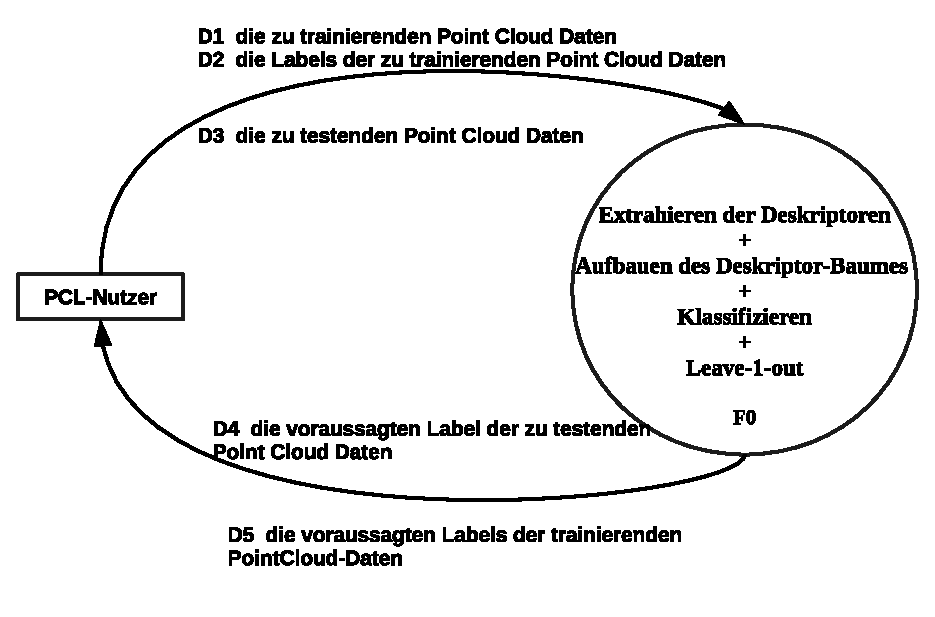
\includegraphics[width=0.7\textwidth]{example_files/log/kontexdiagramm.eps}
  \caption{Kontextdiagramm}\label{fig:digit}

\end{figure}


\begin{table}[h]
\caption{Kontextdiagramm - Daten- und Steuerflüsse}
\centering
\begin{tabular}{p{5.5cm}|p{8cm}}

\hline
\textbf{Datenfluss} & \textbf{Beschreibung}\\
\hline
D1 die zu trainierenden Point Cloud Daten & Die Trainingsdaten im PCD Form, um gute Klassifikatoren zu lernen \\

\hline
D2 die Labels der zu trainierenden Point Cloud Daten  & die Labels für die Trainingsdaten \\
\hline
D3  die zu testenden Point Cloud Daten & Die Testdaten in PCD Form, um die gelernten Klassfikatoren zu testen\\
\hline
D4 die Labels der getesten Point Cloud Daten & die Labels für die getesten Daten , die bei den gelernten Klassifikatoren vorausgesagt werden\\
\hline
D5  die Labels der trainierten Point Cloud Daten & die Labels der Trainingsdaten,  die bei den  gelernten klassifikatoren vorausgesagt werden,  \\
\hline
\end{tabular}
\end{table}

%%%%%%%%%%%%%%%%%%%%%%%%%%%%%%%%%%%%%%%%%%%%%%%%%
\subsection{Datenflussdiagramm - Ebene 1}

Die Aufgabe wird in mehrere Teilaufgaben zerlegt, die Abbildung 2.2 zeigt die
Komposition auf Ebene 1. Die Tabellen 2.2 und 2.3 beschreiben die enthaltenen
Funktionen und Datenflüsse.


\begin{figure}[htb]
  \centering
  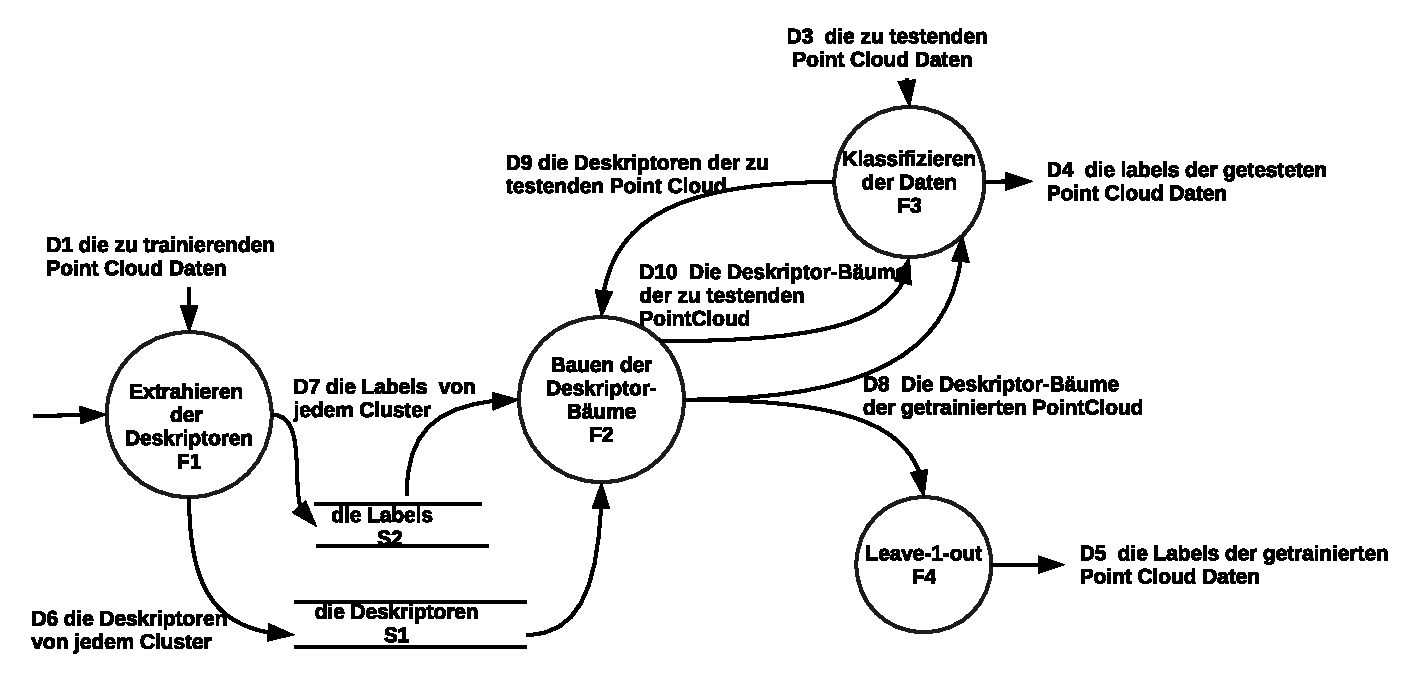
\includegraphics[width=1.0\textwidth]{example_files/log/DE1.eps}
  \caption{Datenflussdiagramm - Ebene 1}\label{fig:digit}
\end{figure}

 \begin{table}[htb]
    \caption{Datenflussdiagramm - Ebene 1 - Funktionen}
     \centering
   \begin{tabular}{p{5.5cm}|p{8cm}}
    \hline
    \textbf{Funktion} & \textbf{Beschreibung}\\
    \hline
     F1  Extrahieren der Deskriptoren& Das Objekt wird in mehrere Cluster unterteilt und die Deskriptoren von jedem Cluster werden berechnet. \\
    \hline
     F2  Bauen des Dekriptor-Baumes &  Der Dekriptor-Baum wird gebaut \\
    \hline
     F3  Klassifizieren der Daten &  
  Die Testdaten werden nach den gelernten Klassifikatoren klassifiziert und erhalten die Prognoselabel    \\
    \hline
     F4  Leave-1-out & die Trainingdaten werden nach den gelernten Klassifkatoren klassifizieren und  erhalten die Prognoselabel\\
    \hline
  \end{tabular}
\end{table}

\begin{table}[htb]
	\caption{Datenflussdiagramm - Ebene 1 - Datenflüsse}
	\centering
	\begin{tabular}{p{5.5cm}|p{8cm}}
		
		\hline
		\textbf{Datenfluss} & \textbf{Beschreibung}\\
		\hline
		D6 die Deskriptoren von jedem Cluster & die Deskriptoren für jeden untergeteilten Cluster \\
		
		\hline
		D7 die Labels  von jedem Cluster  & die Labels für jeden erzeugten Cluster \\
		\hline
		D8  Die Deskriptor-Bäume der getrainierten PointCloud & Die Deskriptor-Bäume von allen Trainingsobjekt\\
		\hline
		D9 die Deskriptoren der zu testenden Point Cloud  & die Deskriptoren für die Test Objekten\\
		\hline
		D10  Die Deskriptor-Bäume der zu testenden PointCloud & Die Deskriptor-Bäume für die Test Objekten  \\
		\hline
	\end{tabular}
\end{table}



%%%%%%%%%%%%%%%%%%%%%%%%%%%%%%%%%%%%%%%%%%%%%%%%%
\subsection{Datenflussdiagramm - Ebene 2 - Funktion 1}

Die im Abschnitt 2.2.2 dargestellten Funtion F1 wird weiter detailliert, um
das Teilsystem deutlich zu machen.

\begin{figure}[h]
    \centering
    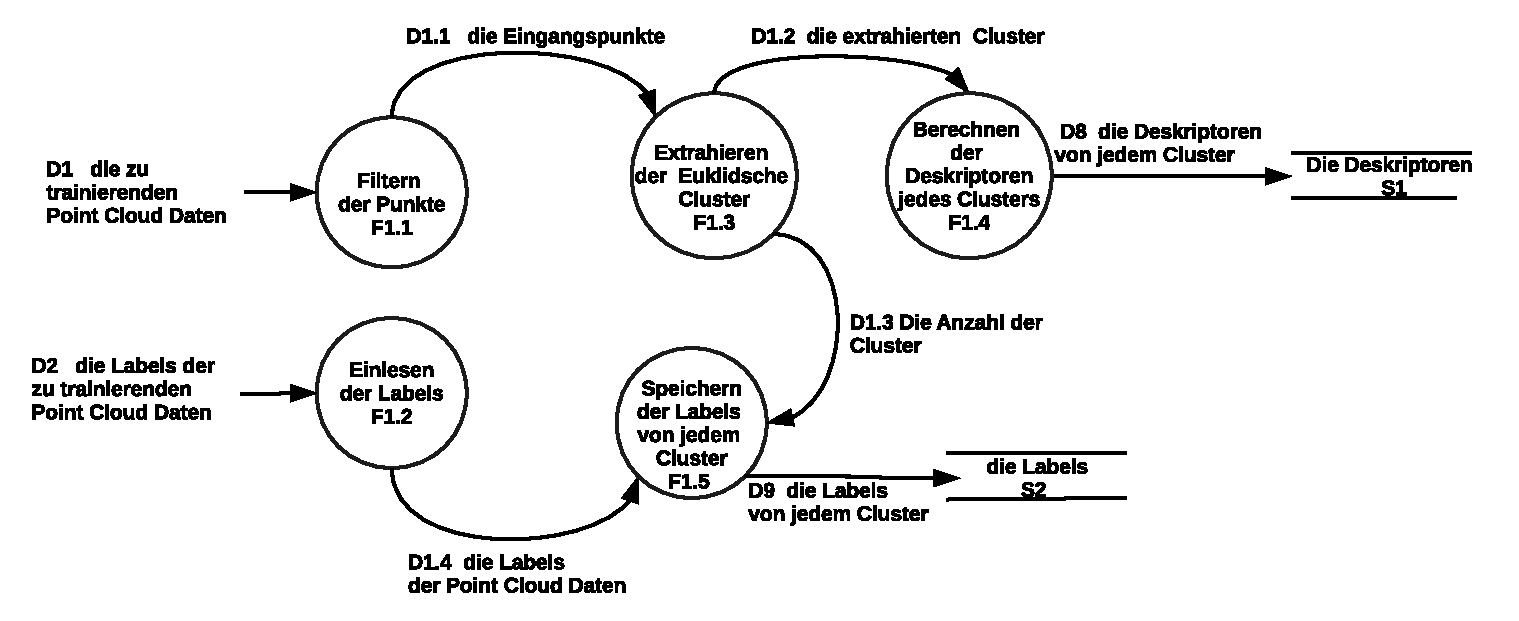
\includegraphics[width=1.0\textwidth]{example_files/log/DE2F1.eps}
    \caption{Datenflussdiagramm - Ebene 2 - Funktion 1}\label{fig:digit}
  \end{figure}
  
  
 \begin{table}[htb]
      \caption{Datenflussdiagramm - Ebene 2 - F1 - Funktionen}
       \centering
     \begin{tabular}{p{5.5cm}|p{8cm}}
      \hline
      \textbf{Funktion} & \textbf{Beschreibung}\\
      \hline
       F1.1  Filtern der Punkte & Die Punkte, die mit höhen Krümmung, sind gefiltert\\
      \hline
       F1.2  Einlesen der Labels & Die Labels der Point Clouds werden heruntergeladet.\\
      \hline
       F1.3  Extrahieren der Euklidsche Cluster &  Das Objekt wird mit bestimmten Euklidschen Distanz unterteilt\\
      \hline
       F1.4  Berechnen der Deskriptoren jedes Clusters &  Die Deskriptoren werden nach den unterteilten Clustern berechnet \\
       \hline
       F1.5  Speichern der Labels  von jedem Cluster &  Entsprechend der Nummer werden die Labels gespeichert \\
       \hline
       
    \end{tabular}
  \end{table}
  
  \begin{table}[htb]
    \caption{Datenflussdiagramm - Ebene 2 - F1 - Datenflüsse}
    \centering
    \begin{tabular}{p{5.5cm}|p{8cm}}
      \hline
      \textbf{Daten- oder Steuerfluss} & \textbf{Beschreibung}\\
      \hline
       D1.1 die Einganspunkte & die Punkte in der PointCloud nach dem Filtern\\
      \hline
       D1.2  die extrahierten Cluster  &  die unterteilten Cluster\\
      \hline
       D1.3 Die Anzahl der Cluster  &  Die Anzahl der Cluster der existierenden Cluster\\
      \hline 
       D1.4 die Labels der Point Cloud Daten &  Die Labels von jeder PointCloud  \\
      \hline
        
    \end{tabular}
  \end{table}
  
  
  


%%%%%%%%%%%%%%%%%%%%%%%%%%%%%%%%%%%%%%%%%%%%%%%%%
\subsection{Datenflussdiagramm - Ebene 2 - Funktion 3}

Die Abbildung 2.4 stellt die Dekomposition der Funktion: F3 dar. Die Tabellen
2.8 und 2.9 beschreiben die enthaltenen Subfunktionen und Datenflüsse.

\begin{figure}[h]
    \centering
    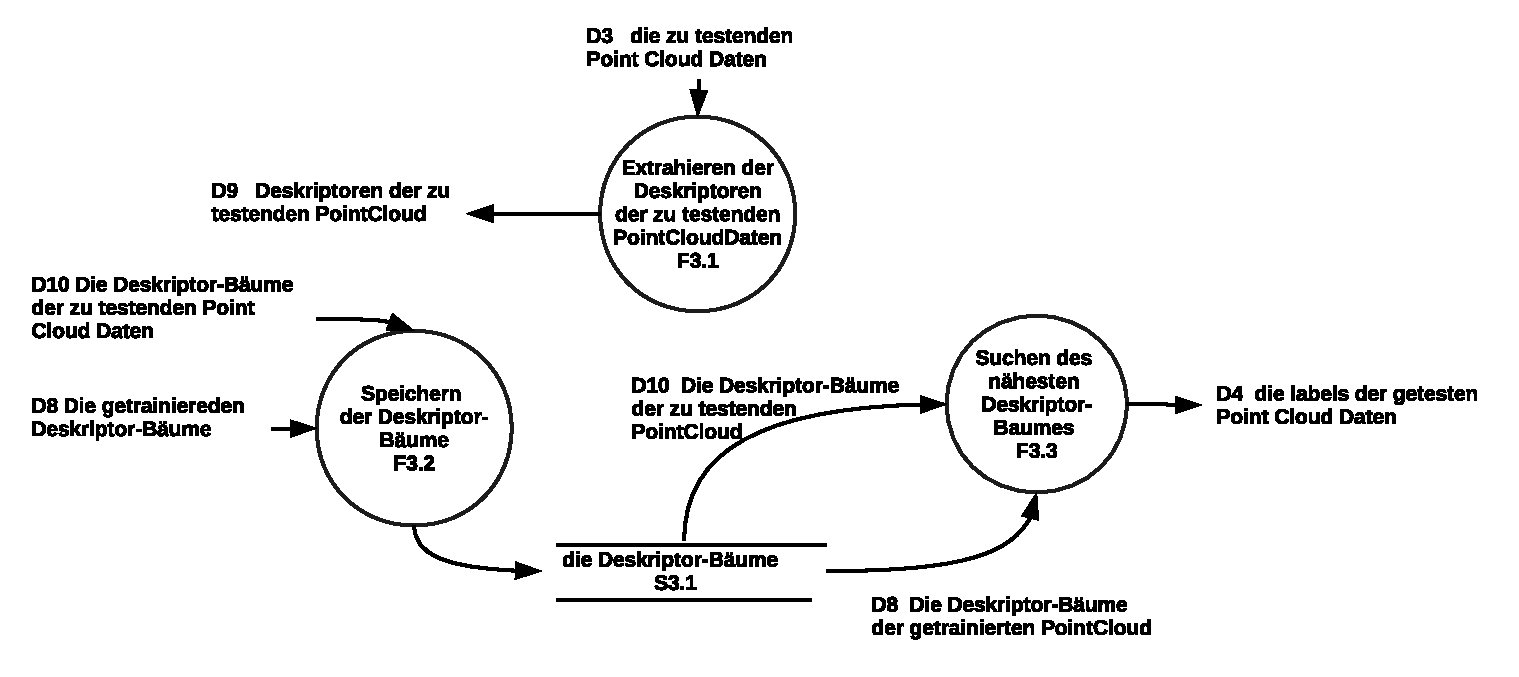
\includegraphics[width=1.0\textwidth]{example_files/log/DE2F3.eps}
    \caption{Datenflussdiagramm - Ebene 2 - Funktion 3}\label{fig:digit}
  \end{figure}
  
  
  
  \begin{table}[htb]
      \caption{Datenflussdiagramm - Ebene 2 -F3 - Funktionen}
       \centering
     \begin{tabular}{p{6.3cm}|p{8cm}}
      \hline
      \textbf{Funktion} & \textbf{Beschreibung}\\
      \hline
       F3.1 Extrahieren der Deskriptoren der zu testenden PointCloudDaten & Die Deskriptoren der Point-Cloud werden als Testdaten berechnet. \\
      \hline
       F3.2  Speichern  der Deskriptor-Bäume  &  Die erzäugten Deskriptorbäume werden gespeichert \\
      \hline
       F3.3 Suchen des nähesten Deskriptor-Baumes  & Die nähsten Deskriptorbäume werden in dem gespeicherten und trainierten Baum gesucht.\\
      \hline
       
       
    \end{tabular}
  \end{table}
  

%%%%%%%%%%%%%%%%%%%%%%%%%%%%%%%%%%%%%%%%%%%%%%%%%
\subsection{Datenflussdiagramm - Ebene 2 - Funktion 4}

\begin{figure}[h]
    \centering
    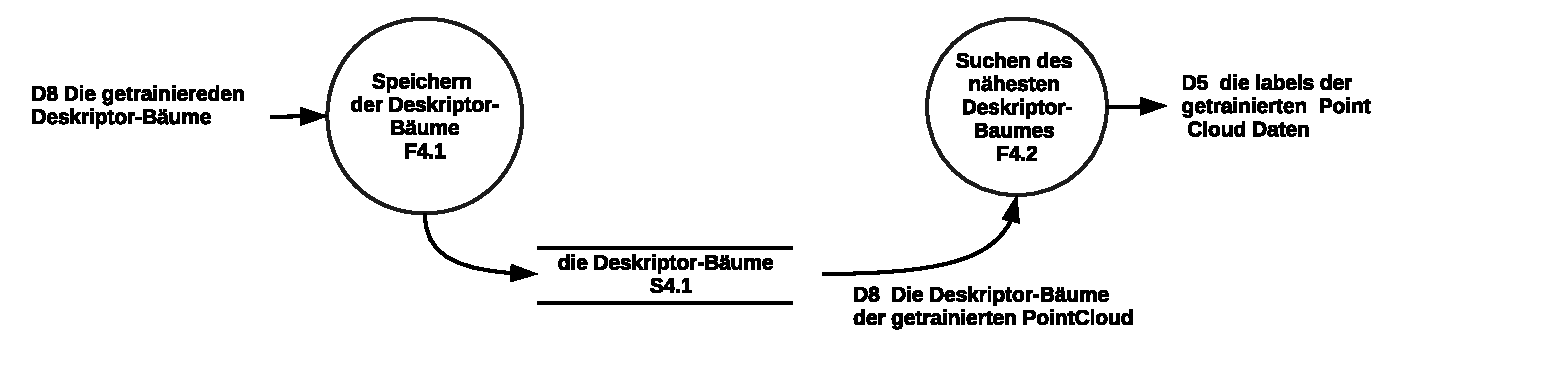
\includegraphics[width=0.95\textwidth]{example_files/log/DE2F4.eps}
    \caption{Datenflussdiagramm - Ebene 2 - Funktion 4}\label{fig:digit}
  \end{figure}



\begin{table}[htb]
    \caption{Datenflussdiagramm - Ebene 2 - F4 - Funktionen}
     \centering
   \begin{tabular}{p{6.3cm}|p{8cm}}
    \hline
    \textbf{Funktion} & \textbf{Beschreibung}\\
    \hline
     F4.1   Speichern  der Deskriptor-Bäume & Die erzäugten Deskriptorbäume werden gespeichert\\
    \hline
     F4.2   Suchen des nähesten Deskriptor-Baumes  &Die nähsten Deskriptorbäume werden in dem gespeicherten und trainierten Baum gesucht. \\
    \hline
    
  \end{tabular}
\end{table}








%%!TEX root = /Users/stefan/Entwicklung/de.tud.et.ifa.latex.ifathesis/example.tex
%*******************************************************************************
% * Copyright (c) 2006-2013 
% * Institute of Automation, Dresden University of Technology
% * 
% * All rights reserved. This program and the accompanying materials
% * are made available under the terms of the Eclipse Public License v1.0 
% * which accompanies this distribution, and is available at
% * http://www.eclipse.org/legal/epl-v10.html
% * 
% * Contributors:
% *   Institute of Automation - TU Dresden, Germany 
% *      - initial API and implementation
% ******************************************************************************/

%%%%%%%%%%%%%%%%%%%%%%%%%%%%%%%%%%%%%%%%%%%%%%%%%%%%%%%%%%%%%%%%%%%%%%
%%%%%%%%%%%%%%%%%%%%%%%%%%%%%%%%%%%%%%%%%%%%%%%%%%%%%%%%%%%%%%%%%%%%%%
\chapter{Grundlage}
\label{sec:AllgemeineHinweiseZurVorlage}

Das Kapitel stellt die wirtschaftswissenschaftliche Grundlage.



\section{Werkzeug}
In diesem Abschnitt   werden die  in dem recherchierten Projekt verwendeten Werkzeugen kurz eingeführt:
    \begin{compactitem}
       \item \verb-das KUKA youBot-,  omnidirektionalen mobilen Plattfor  mit vier Mecanum  Rädern,  ein fünfachsiger Roboterarm mit Zweifinger-Greifer;
       \item \verb-Robot Operating System-, ein  Robotik Software Framework . 
       \item \verb-Gazebo-,   Simulationsumgebung 
       \item \verb-Matlab2015: Robotics System Toolbox-
       \item \verb-RVIZ-: eine gute Alternative für die Simulation der Prozessvisualisierung
       \end{compactitem}





%%%%%%%%%%%%%%%%%%%%%%%%%%%%%%%%%%%%%%%%%%%%%%%%%%%%%%%%%%%%%%%%%%%%%%
\section{KUKA youBot Hardware Schnittstellen}
\label{sec:install}
%%%%%%%%%%%%%%%%%%%%%%%%%%%%%%%%%%%%%%%%%%%%%%%%%%%%%%%%%%%%%%%%%%%%%%




\subsection{KUKA youBot Hardware}

\subsubsection{KUKA youBot Base}
Die KUKA youBot Base ist eine omnidirektionale mobile Plattform mit vier Mecanum  Rädern. Abbildung 3.1 zeigt das angeschlossene Basis (Koordinate) Rahmen, wie es in der KUKA youBot API verwendet werden.

\begin{figure}[htbp]
  \centering
  \includegraphics[width=0.6\textwidth]{example_files/youbotbase.pdf}
  \caption{Überblick über die KUKA youBot Basis}\label{fig:digit}
\end{figure}
\subsubsection{KUKA youBot Arm}

Der KUKA youBot Arm ist ein fünfachsiger Roboterarm mit Zweifinger-Greifer.Die Roboter-Manipulator hat sechs Links,die von 5 betätigten Drehgelenke verbunden.Die Drehachse der Gelenk 1 und 5 ist die z-Achse in dem Rahmen dargestellt ist,
für gemeinsame 2,3 und 4 ist die Drehachse die y-Achse(sieh Abbildung 3.2).

\begin{figure}[htbp]
  \centering
  \includegraphics[width=0.6\textwidth]{example_files/youbotarm.pdf}
  \caption{Überblick über die KUKA youBot Arm}\label{fig:digit}
\end{figure}


%%%%%%%%%%%%%%%%%%%%%%%%%%%%%%%%%%%%%%%%%%%%%%%%%%%%%%%%%%%%%%%%%%%%%%
\subsection{KUKA youBot API}
%%%%%%%%%%%%%%%%%%%%%%%%%%%%%%%%%%%%%%%%%%%%%%%%%%%%%%%%%%%%%%%%%%%%%%
Die KUKA youBot API ist die Programmierschnittstelle, über die der Entwickler Zugriff 
die KUKA youBot Hardware zugriffen und steuern,kann  für den Roboter als High-Level Treiber angezeigt werden.
%%%%%%%%%%%%%%%%%%%%%%%%%%%%%%%%%%%%%%%%%%%%%%%%%
\subsubsection{Einführung}
The KUKA youBot driver besteht aus zwei Teilen:
\begin{compactitem}
  \item \verb-EtherCAT driver- Auf der untersten Niveau der Steuerung alle Aktoren der KUKA youBot über das EtherCAT-Protokoll angesteuert werden. Dieses Protokoll verwendet Standard Netzwerk Hardware wie Ethernet-Adapter,entsprechenden RJ45-Stecker und Netzwerkkabel EtherCAT Master und Slaves zu verbinden und die Kommunikation zwischen ihnen herstellen
  \item \verb-KUKA youBot API- Auf der Oberseite des EtherCAT-Treiber-Stack gibt es eine zweite Softwareschicht  \{ der KUKA youBot API  \{ die youBot Plattform zu befehlen. Es baut SOEM EtherCAT Treiber auf  und bietet zusätzliche Funktionalität relevant Plattform Kinematik.
  
  Derzeit bietet diese Bibliothek die grundlegenden Funktionalitäten, der kartesischer Geschwindigkeiten der Basis einzusetzen, Odometriedaten von Motorgebern zu lesen,usw.Mit API können folgende GelenkDate gemseen und gesteuert werden:
   \begin{compactitem}
    \item \verb-Geschwindigkeit-
    \item \verb-Position-
    \item \verb-Strom-
    \item \verb-PWM-
    \end{compactitem}
  
  \begin{figure}[htbp]
    \centering
    \includegraphics[width=0.8\textwidth]{example_files/driver.png}
    \caption{Überblick über die youBot driver}\label{fig:digit}
  \end{figure} 
\end{compactitem}





%%%%%%%%%%%%%%%%%%%%%%%%%%%%%%
\subsubsection{C++ API Dokumentation}
Der youBot driver besteht aus C++ Klassen, die Low-Level-Zugriff auf die KUKA youBot Hardware zur Verfügung stellen.
\\
Es gibt drei Hauptklassen in der youBot API. Diese sind:
\begin{compactitem}
 \item \verb-YouBotManipulator- Klasse,die die Aggregation mehrerer Gelenke und einem Greifer von youBot darstellt.
 \begin{figure}[htb]
       \centering
       \includegraphics[width=0.8\textwidth]{example_files/mani.png}
       \caption{YouBotManipulator}\label{fig:digit}
 \end{figure} 
 \\
 \item \verb-YouBotBase- Klasse,die die youBot Basisplattform darstellt.
 \begin{figure}[htb]
     \centering
     \includegraphics[width=1.0\textwidth]{example_files/jointbase.png}
     \caption{YouBotBase}\label{fig:digit}
 \end{figure}
 \item \verb-YouBotJoint- Klasse, die die Gelenke darstellt, welche sowohl der Manipulator und die Basis bilden.
 \begin{figure}[htb]
      \centering
      \includegraphics[width=1.0\textwidth]{example_files/joint.png}
      \caption{YouBotJoint}\label{fig:digit}
  \end{figure} 
\end{compactitem}

Jedes youBot Gelenk wird als youBot::YouBotJoint Klasse in der API vertreten. In diesem Stadium machen die API keinen Unterschied,ob es ein Basisgelenk oder ein Manipulator Gelenk.
\\youBot::YouBotBase und youBot::youBotManipulators sind aggregierte Klassen, die den Zugriff auf eine bestimmte gemeinsame Instanz durch youBot::youBotJoint erlauben. 
 
\subsubsection{Klassen für set/get Joint Werte}
Um Sollwerte zu setzen und zu erhalten oder einige Sensoren von Gelenken zu lesen, wird die Klasse  youBot::JointData verwendet.Im diesem Project werden followen Data Klassen verwendet:
    \begin{compactitem}
    \item \verb-youbot::JointSensedAngle-
    \item \verb-youbot::JointSensedCurrent-
    \item \verb-youbot::JointSensedTorque-
    \item \verb-youbot::JointSensedVelocity-
    \item \verb-youbot::JointAngleSetpoint-
    \item \verb-youbot::JointCurrentSetpoint-
    \item \verb-youbot::JointTorqueSetpoint-
    \item \verb-youbot::JointVelocitySetpoint-
    \end{compactitem}


Weiterhin können alle GelenkParameter können auch kongiguriert, z.B  PID-Regler Parameter.
da wird die  Klasse youBot::JointParameter verwendet, z.B youbot::IParameterFirstParametersPositionControl
 
 

\begin{figure}[htb]
    \centering
    \includegraphics[width=0.8\textwidth]{example_files/jointbm.png}
    \caption{Zustandsmaschine für youBot Basis und Zustandsmaschine für youBot Arm}\label{fig:digit}
\end{figure} 


%%%%%%%%%%%%%%%%%%%%%%%%%%%%%
\section{Robotik Software Framework}
\label{sec:BefehleUndUmgebungen}

ROS (Robot Operating System) stellt Bibliotheken und Werkzeuge zur Verfügung, welche Softwareentwicklern helfen Roboteranwendungen zu erstellen. ROS kann als Robotik Software Framework für KuKa youBot verwendet.
 

\subsection{Einführung in ROS}

Das Robot Operating System (ROS) ist ein Open-Source-Projekt, dass von der Firma Willow Garage entwickelt und in regelmäßigen Abständen als Distribution veröffentlicht wird. Vielmehr als ein Roboterframework versteht sich ROS als ein Meta-Betriebssystem für Roboter, das unter Linux und Mac OS X betrieben werden kann. Es bietet hierführ betriebssystemähnliche Dienste, wie Hardwareabstraktion, eine Nachrichtensteuerung zwischen Prozessen, Treiber für Hardwarekomponenten, Paketmanagement und Tools für häufig benötigte Aufgaben.
\\Durch die Verwendung von XML-RPC, welches für viele Programmiersprachen implementiert wurde, können Softwarekomponenten zum Beispiel in C++, Python,Octave, Java, Lua oder LISP erstellt und trotzdem gemeinsam verwendet werden.
Die Komponenten werden als Nodes bezeichnet und sind ohne spezielle Ausführungslogik einzeln verwendbar. Auch die Kommunikation wird sprachenneutralgehalten, indem eine einfach-gehaltene Schnittstellendefinitionssprache verwendet
wird. Die Nachrichtendefinitionen, die in dieser IDL beschrieben sind, werden automatisch in die jeweiligen Programmiersprachen übersetzt.
Ein ROS-System besteht aus den im Folgenden näher erläuterten fundamentalen Konzepten:
\begin{description}
    \item[Packages]Software in ROS wird in Paketen organisiert.
  Ein Paket könnte ROS Knoten, eine ROS-unabhängige Bibliothek, ein Datensatz, Konfigurationsdateien , eine Drittanbieter -Stück Software, oder irgendetwas anderes, das ein nützliches Modul logisch darstellt, enthalten.
  
  \item[Stacks] $:$  Mehrere Pakete , die mit einigen gemeinsamen Ziel
  miteinander kombiniert werden , werden als Stacks genannt.
  
  \item[Nodes] $:$ 
  In ROS werden die eigenständigen Ausführungseinheiten, aus denen sich das gesamte System
  zusammensetzt, als\emph{Nodes} bezeichnet.
  
  
   Die Instanz eines Nodes ist ein Softwareprozess
  der Berechnungen innerhalb seines eigenen Speicherbereiches ausführt. Im Sinne des CBSE
  entspricht ein Node also einer Komponente.
  Nodes können sich zur Laufzeit am System an- und abmelden. Wie bereits erwähnt kann
  die Implementierung eines Nodes in jeder Programmiersprache erfolgen, für welche eine
  entsprechende Bibliothek (ROS-Library) existiert.
  
  \item[Message]  $:$ In einem ROS-System kommunizieren die Nodes untereinander über Messages. Messages
  sind einfache Datenstrukturen, die typisierte Felder enthalten. Zur Spezifikation von Messages
  definiert ROS eine IDL, mit welcher die typisierten Felder in einer Textdatei (message
  file) beschrieben werden. Jeder so definerte Messagetyp stellt selbst wiederum einen Datentyp
  dar, der als Typ eines Feldes in einer anderen Message verwendet werden kann.
  
  \item[Topics]  $:$ Der Transport einer Message im ROS Communication Layer erfolgt nach dem PublishSubscribe-Modell.
  Ein Node versendet Nachrichten eines bestimmten Messagetyp indem
  er sie unter einem Topic veröffentlicht. Alle Nodes die an diesen Nachrichten interessiert
  sind, können diese über das Topic abonnieren. Jede neue Message, die auf einem Topic ver-
  öffentlicht wird, wird daraufhin allen abonnierenden Nodes zugestellt.
  Topics sind also eindeutige Bezeichnungen, mit denen ein Nachrichtenkanal innerhalb des
  ROS-Systems identifiziert werden kann. Ein Topic ist dabei immer fest an einen bestimmten
  Messagetyp gebunden.
  
  \item[Service] $:$ Über Services ist eine synchrone Kommunikation nach dem Client/Server-
  Modell möglich. Hierfür bietet ein Node einen Service an, den ein anderer Node
  anfordert und anschließend auf die Antwort wartet. Im Ge-
  gensatz zu Topics kann hier immer nur ein Node einen be-
  stimmten Service anbieten, der von beliebig vielen Nodes angefordert wird.
\end{description}





\subsection{Die Kommunikation von ROS}
ROS bietet folgende Kommunikationsarten:
\begin{enumerate}

  \item \verb|ROS Topics Kommunikation|
  
   Eine Möglichkeit zur Kommunikation zwischen den Nodes innerhalb eines ROS-Systems
   ist das Versenden und Empfangen von Datenpaketen mittels Nachrichten nach dem Prinzip
   des Publish-Subscribe-Modells [ROSa].
   Bevor zwei Komponenten eines ROS-Systems Nachrichten austauschen können, muss ein
   entsprechender Nachrichtenkanal zwischen ihnen hergestellt werden. Dies wird vom ROS
   Communication Layer übernommen, sobald sich mindestens eine Komponente als Sender
   (Publisher) und eine als Empfänger (Subscriber) eines bestimmten Nachrichtentyps beim
   ROS Master-Node angemeldet hat. Hierfür gibt der Publisher bei seiner Registrierung neben
   dem Datentyp der Nachrichten (Message) die er versenden möchte, auch eine systemweit
   eindeutige Kennung, das sogenannte Topic, an. Ein anderer Node kann sich darauf für die
   Abonnierung des Topics beim Master registrieren. Er wird damit zu einem Subscriber des
   Topics. Der Subscriber gibt bei seiner Registrierung auch die Referenz einer Funktion an,
   welche die Nachrichten entgegennimmt. Diese sogenannte Callback-Funktion wird immer
   dann von der Middleware aufgerufen, sobald eine neue Nachricht unter dem registrierten
   Topic versandt wurde. Dem Callback wird eine Kopie dieser Nachricht als Parameter übergeben
   
  
  
  
  \item \verb|ROS Services Kommunikation|
  
  Das Publish-Subscribe-Modell ist eine sehr flexible Kommunikationstechnik, doch wie in
   Abschnitt 2.2 beschrieben handelt es sich dabei um eine unidirektionale Form der Kommunikation.
   Um auch bidirektionale Interaktionen zwischen den Nodes eines ROS-Systems
   abbilden zu können, wurde das Konzept des ROS Service eingeführt [ROSa].
   
   ROS-Services bilden ein dynamisches Remote-Procedure-Call (RPC) Grundgerüst. Die RPC-
   Kommunikation erfolgt synchron. Der Aufrufer des Service wird so lange blockiert, bis seine An-
   frage mit einer Ergebnisnachricht beantwortet worden ist.
   Auch hier meldet ein Node einen angebotenen Dienst beim Master-Node mit einem eindeutigen Namen
   (Service) an. Gleichzeitig übergibt er eine Referenz auf die, bei einem Aufruf des Dienstes,
   auszuführende Prozedur (Callback). Alle Nodes die einen bestimmten Dienst in Anspruch nehmen möchten, müssen dies ebenfalls dem Master melden. Ein Client kann diesen Dienst nutzen, indem er einen entsprechenden Aufruf an die ROS-Middleware absetzt.  
   
   
  \item \verb|ROS Parameter-Server Kommunikation|
  
  Der Parameter-Server ist ein zentraler Service im ROS-System und Teil des ROS Masters.
   
   Parameter sind nicht für den Nachrichtenaustausch zwischen Nodes konzipiert, sondern
   werden zur systemweiten Verbreitung statischer Daten genutzt, die vorwiegend der Kon-
   figuration und der Initialisierung von Nodes dienen. Die Werte der Parameter können zur Laufzeit von Nodes gespeichert und abgerufen werden und werden in Form assoziativer
   Datenfelder (Schlüssel-Werte Paare) auf dem Parameter-Server verwaltet.
   
   Auch das Hinzufügen und Löschen von Parametern ist zur Laufzeit möglich. 
   Im Gegensatz
   zu ROS Topics und ROS Services handelt sich es beim Parameter-Server also nicht um
   ein klassisches Interface, dessen Struktur durch eine Spezifikation definiert werden muss.
   Vielmehr handelt es sich beim Parameter-Server um einen globalen Speicherbereich, auf
   welchen flexibel von allen Nodes zugegriffen werde kann.
  
  
  \end{enumerate}   

 

 
 
 \subsection{Launchfiles}


Jeder Node kann über die Kommandozeile einzeln gestartet und konfiguriert werden. Je nach Robotersystem und Aufgabe kann das schnell komplexe Züge annehmen, da für ein System beliebig viele Nodes gestartet und konfiguriert werden können. Das System besteht letztlich aus allen Komponenten, wie Hardwaretreibern, zugrunde liegenden Funktionen, wie Navigation und Hindernisvermeidung,Bilderkennung oder Lokalisierung und der Implementierung der eigentlichen Aufgabe. Ein solches System muss in der Regel mehr als nur einmal ausgeführt werden.
Damit bei einem erneuten Aufruf des gesamten Softwaresystems nicht alles manuell erneut gestartet werden muss, existiert in ROS das Konzept der Launchfiles, die Start- und Konfigurationsinformationen beinhalten und über das Tool roslaunch gestartet und abgearbeitet werden. Sie stellen dabei eine XML-Beschreibung des Berechnungsgraphen dar und ermöglichen auch die Parametrisierung der Nodes sowie eine Beschreibung des Robotersystems auf dem das Softwaresystem ausgeführt werden soll. Beim Ausführen eines Launchfiles werden die in ihm beschriebenen
Nodes auf einem optional spezifizierten Host-System instantiiert und können zentral beendet werden. Mehrere Instanzen eines Nodes können durch verschiedene Namen und Namespaces gestartet werden. Auch Parameter können mehrfach in einem Launchfile vorkommen, allerdings wird der Parameter dem letzten Eintrag nach auf dem Parameterserver gespeichert.



Die Elemente in XML-Dateien werden Tags genannt. Die Launchfile-Tags werden sowohl inhaltlich als auch strukturell auf verschiedene Weisen genutzt. Sie besitzen alle unterschiedliche Pflichtattribute und zusätzliche optionale Attribute, bei denen, falls man sie nicht setzt, Default-Werte angenommen werden.


Jeder Tag besitzt zusätzlich zu den im weiteren Verlauf aufgeführten Attributen
in jedem Fall noch die folgenden beiden Attribute als optionale Attribute:
\begin{compactitem}
 \item  if=’value’, wertet den Tag beim Start aus, falls ’value’ den Wahrheitswert
 Wahr annimmt
 \item unless=’value’, falls ’value’ nicht Wahr ist, wird der Tag beim Start beachtet
 
\end{compactitem}

\begin{description}

\item[launch] Jeder Launchfile beginnt mit einem <launch>-Tag und schließt mit einem
</launch>-Tag. Weitere Funktionen hat der <launch>-Tag nicht.

\item[text]


\item[Param]
Parameter, die durch diese Tags angegeben werden, werden auf dem Parameter-
Server gespeichert bevor ein Knoten gestartet wird. Auch für <param>-Tags exis-
tieren verschiedene Benutzungsszenarien, mit denen Parameter auf dem Server
342.4. Launchfiles
gespeichert werden können. In jedem Fall muss ein name=’namespace/name’-
Attribut gesetzt werden, anschließend muss eine der folgenden Optionen gewählt
werden:
\item[rosparam]


\end{description}








%%%%%%%%%%%%%%%%%%%%%%%%%%%%%
\section{Gazebo}

Gazebo ist eine Simulator, der speziell für den Einsatz in der Robotik entwickelt und für die Unterstützung im Entwicklungsprozess neuer Algorithmen für Roboterplattformen konzipiert wurde. Es können in Gazebo mehrere Roboter, deren Sensoren und deren Interaktion mit der Umgebung simuliert und dargestellt werden.\\ Die Interaktionen zwischen Objekten wird über eine Physikengine, welche auf der Starrkörperphysik basiert, gelöst. Gazebo läuft unter Linux und verwendet als Engine die ODE (Open Dynamics Engine). Diese wird neben Gazebo auch in diversen anderen Robotersimulationen verwendet, u.a. in V-REP(Virtual-Robotic Expermentatial Plattform) und Webbots (vgl. [2]). Im Jahr 2009 wurde ROS (Robot Operating System) von Willow Garage in Gazebo integriert (vgl. [1]), somit kann man auf die Daten der Simulation in der ROS Kommunikationsstruktur zugreifen und diese verarbeiten. Auf die Kommunikation und ROS(in Abschnitt 3.4.1) wird später eingegangen. 

Gazebo kann  für unterschiedlichen Aufgaben verwendet,z.B:
    \begin{compactitem}
    \item \verb|Rapid Prototyping|:Parallele Entwicklung von Hardware und Software (u.a. mit Schnittstellen
    zu ROS und Solidworks).
    \item \verb|Reverse Engineering|:Zur Bestimmung und Abbildung der Funktionalität komplexer Systeme,
    bei denen nicht auf Anhieb gesagt werden kann, wie diese funktionieren. Ein Beispiel
    hierfür ist der Segway. Ein einfacher simulierter
    Zweirad-Antrieb hätte den realen Antrieb nicht korrekt wieder gegeben, da dieser durch
    Kippen und Neigen des Segways selbst gesteuert wird.
    \item \verb|Algorithmus-Design|:Testen von Algorithmen in passenden Szenarien.
    \item \verb|Sensortests|:Diese erfordern normalerweise echte Hardware.
    \item \verb|Szenarien-basierte Tests|:Testen von Roboterverhalten und -verfahren in verschiedenen
    Situationen und Umgebungen.
    \end{compactitem}

\subsection{Aufbau von Gazebo}

Gazebo besteht aus zwei Hauptkomponenten: dem Gazebo-Server und dem Gazebo-Client. Der
Gazebo-Server stellt die eigentliche Funktionalität von Gazebo bereit. Der Gazebo-Client ist für
die Darstellung der Simulation und die Benutzer-Interaktion zuständig. Die Funktionalität dieser
beiden Komponenten wird durch verschiedene Bibliotheken gewährleistet (vgl. Abbildung 2.5).
Als Basis jeder Simulation dient die Definition einer Systemwelt. Diese kann den gewünschten
physikalischen Gegebenheiten angepasst und es können beliebige Gegenstände, wie z.B. Roboter
oder Hindernisse, eingefügt werden. Die Steuerung und Funktionalität von Objekten wird
durch Plugins ermöglicht. Alle Elemente in Gazebo werden durch das Simulation Description
Format (SDF) beschrieben, auf das im weiteren Verauf der Arbeit näher eingegangen wird.

\subsection{Kommunikation mittels ROS}

Da mit Gazebo die erzeugten Daten nicht ausgewertet werden können, werden sie
über das ROS-Netzwerk dem Programm Matlab verfügbar gemacht.
Die Kommunikation innerhalb der ROS-Umgebung läuft über Nachrichten, sogenannte
Topics. Im Netzwerk integrierte Anwendungen können diese Nachrichten
senden und empfangen. Die Kommunikation wird über einen roscore gesteuert. Dieser
stellt den Master im Netzwerk dar. Ein Teilnehmer kann sich mit dem Master
zu verbinden, um Nachrichten zu empfangen und senden. Man kann somit eine auf
ROS basierende Robotersteuerung in das Netz als Knoten integrieren und mittels
Gazebo den Arbeitsablauf realitätsnah simulieren und somit optimal auswerten.



\subsection{Visualisierung}

Gazebo bietet eine API zur Programmierung eigener Steuerungs- und Ausgabekonsolen für die Erweiterung der vorhandenen GUI. Auf diese Möglichkeit wird zugunsten der Verwendung von RVIZ verzichtet. RViz ist ein 3D-Visualisierungstool von ROS, das auch für die visuelle Steuerung und Darstellung des realen Roboters verwendet wird. Es ermöglicht die Darstellung des Robotermodells, der Sensordaten und der grafischen Auswahl von Navigationszielen über die Umgebungskarte. Die benötigten Informationen werden über ROSNachrichtenströme (Topics) ausgetauscht.





RViz ist ein 3D-Visualisierungstool von ROS, das für die visuelle Steuerung und Darstellung des realen Roboters und seiner Sensoren verwendet wird (vgl. Abschnitt 3.2.4). Da RViz die benötigten Informationen über ROS-Topics austauscht und der Scitos sowie der simulierte Roboter
die gleichen ROS-Module nutzen, erfolgt die grafische Steuerung ebenfalls über RViz. Für die Repräsentation des Roboters in RViz wird das URDF-Modell des Scitos verwendet, da in RViz das SDF-Format nicht unterstützt wird

Je nachdem welche Anzeige- und Steuerungs-Plugins in RViz geladen werden, variieren die
abonnierten und angebotenen Topics. In Bezug auf die Simulation müssen für die Verwendung
von RViz keine zusätzlichen Schnittstellen bereitgestellt werden, die über die vorher beschriebe-
nen Funktionen hinausgehen.


 
%%%%%%%%%%%%%%%%%%%%%%%%%%%%%
\section{Robotics System Toolbox von Matlab2015}
Robotics System Toolbox  bietet Algorithmen und Hardware-Konnektivität für Anwendungen und Entwicelung von autonomen mobilen Robotik.Toolbox-Algorithmen umfassen Kartendarstellung , Routenplanung und Pfad für Differentialantrieb Roboter.Das System Toolbox bietet eine Schnittstelle zwischen MATLAB und Simulink und dem Robot Operating System (ROS),so dass es möglich ist,  Anwendungen auf ROS-fähigen Roboter und Roboter-Simulatoren wie Gazebo zu testen und zu verifizieren.Es unterstützt C ++ Code-Generierung, so dass  man einen ROS Knoten aus einem Simulink-Modell generieren kann.




Ein ROS-Netzwerk besteht aus einem einzigen ROS-Master und mehrere ROS-Knoten. Jeder Knoten muss mit dem ROS Master registrieren, sodass  es in der Lage  mit dem Rest des Netzes  kommunizieren könnte.MATLAB können die ROS-Master starten oder der Master kann außerhalb MATLAB gestartet werden (beispielsweise auf einem anderen Computer). Alle ROS Knoten registrieren mit dem Master und geben 
die Netzwerkadresse an, wo sie erreicht werden können.

Folgend sind die Schritte, um mit ROS im Matlab zu arbeiten

\begin{compactitem}
\item \verb|Verbindung mit einem ROS-Netzwerk|

Um  einem ROS-Netzwerk  zu verbinden, könnte sich der ROS-Master in MATLAB erstellen lassen oder eine vorhandene ROS Master anschließen lassen. In beiden Fällen wird MATLAB auch einen eigenen ROS Knoten (das so genannte MATLAB "globalen Knoten") mit dem Master erstellt und registriert.




\item \verb|Datenaustaucshen|

Sobald die Verbindung steht, MATLAB tauscht Daten mit anderen ROS-Knoten durch Publisher, Subscribers, and Services.

\item \verb|Unterbrechen mit dem ROS-Netzwerk|

MATLAB "globalen Knoten" wird  mit dem ROS-Netzwerk unterbrecht durch des Aufrufes der Funktion \emph{rosshutdown}.

\end{compactitem}



\chapter{Analyse der verwendet Arbeiten}



Im vorherigen Abschitt wurde die wirtschaftswissenschaftliche Grundlage für diese Arbeit vorgestellt,wird in diesem Kapitel die schon feitig ROS Schnittstellen von   KUKA youBot ROS Wrapper und  KUKA youBot Gazebo Wrapper ausführlich erläutert.

\section{KUKA youBot ROS Wrapper}

\subsection{Überblick}
Nachdem ROS als Vermittlungsschicht und die eingesetzten Hardwarekomponenten des Roboters im Kappitel 3 beschrieben wurden, sollen im folgenden zentrale Knoten des KUKA youBots beschrieben werden, welche zur Abstraktion der Hardware eingesetzt werden.Es trägt den Name \\ \verb|youbot_driver_ros_interface| , die  zu dem ROS Wrapper für KUKA youBot API gehört.

Die KUKA youBot ROS Wrapper stellt eine Schnittstelle der KUKA youBot API ( im \verb|youbot-driver| Paket implementiert ) an den ROS Rahmen.In diesem Arbeit wird an den ROS Indigo Rahmen gearbeitet, deshalbt wird ROS Indigo Wrapper  für KUKA youBot in Ubuntu 14.04 installiert.

Mit dem youBot ROS Wrapper  können  die Basis und den Arm des KUKA youBot gesteuert werden. Die Steuerungdaten sollen Narichten unter die von youBot ROS Wrapper gebietet Topic gesendet werden. Damit spielt Narichten in diesem Arbeit aucho eine wichtigen Rolle.
Die Nachrichten, die für youBot driver verwendet werden,  reflektieren verschiedenen Abstraktionsebenen. Eine Ebene ist die \verb|Gelenk Ebene|,
in denen Gelenkpositionen in [RAD] und Gelenkgeschwindigkeiten in [rad / s] eingestellt oder empfangen werden.Wenn man Nachrichten an den Gelenken senden möchte, müssen die richtigen Namen verwendet werden, sonst wird die Nachricht ignoriert.Die Gelenknummern und die entsprechenden Gelenknamen sind in unteren Tabelle aufgelistet.
\\Die andere Ebene,auf dem die mobile Basis Nachrichten bietet,ist\\ \verb|kinematischen| \verb|Ebene|. Über den Nachrichtentype \emph{Twist} einer Richtungs- und Drehgeschwindigkeit  ist die Basis im freien Raum steuerbar.

   \begin{table}[h]
       \caption{Joint names used for the ROS messages}
        \centering
       \begin{tabular}{l|l}

          \hline
          \textbf{Joint} & \textbf{Joint name}\\
           \hline
            Wheel \#1 & wheel\_joint\_fl \\
           \hline
            Wheel \#2 & wheel\_joint\_fl \\
            \hline
            Wheel \#3 & wheel\_joint\_bl \\
            \hline
            Wheel \#4 & wheel\_joint\_br \\
            \hline
            Arm joint \#1 & arm\_joint\_1 \\
            \hline
             Arm joint \#1 & arm\_joint\_1 \\
            \hline
             Arm joint \#2 & arm\_joint\_2 \\
            \hline
             Arm joint \#3 & arm\_joint\_3 \\
             \hline
             Arm joint \#4 & arm\_joint\_4 \\
            \hline
             Arm joint \#5 & arm\_joint\_5 \\ 
             \hline
             Joint for the left gripper finger & gripper\_finger\_joint\_l   \\      
             \hline
              Joint for the right gripper finger & gripper\_finger\_joint\_r  \\                            

          \hline
        \end{tabular}
   \end{table}
  
 Nachrichtentype: \verb|brics_actuator/JointPositions|
         
         der Ausschnitt der Nachrichten type im Detail:
         
         \begin{compactitem}
            \item  \verb|brics_actuator/Poison poisonStamp|
                     \\  \verb|string originator|  
                     \\  \verb|string description|
                     \\  \verb|float32 	qos|
            \item   \verb|brics_actuator/JointValue[] positions|
                     \\  \verb|time timeStamp|
                     \\  \verb|string joint_uri|
                     \\  \verb|string unit|
                     \\  \verb|float64 value|         
         \end{compactitem}
         
         
         dien \emph{joint uri} enthältet die Armgelenken 

\subsection{KUKA youBot ROS Wrapper Kommunikation}  
Wie im Abschnitt 3.3.2 dargestellt, dass Publisherm, Subsriver, Client und Server vier unterschiedliche Typen von Schnittstelen sind, die einem Node als Kommunikationspunkte nach außen dienen,  werden  dann die Schnittstellen von youBot Wrapper in diesen vier Kommunikaitonstypen dargestllet, die im Kappitel 4.1.2.1 bis 4.1.2.4 ausführlich erläutet werden. 

Die KUKA youBot ROS Wrapper bietet eine  Zuordnung zwischen den ROS-Nachrichten und KUKA youBot (oodle) API Methodenaufrufe.
Er veröffentlicht zu verschiedenen Topics  und bietet verschiedene Services für die Kommunikation mit dem youBot.
Es kann die Basis und einen oder zwei Arme für die Kommunikation zu initialisieren,dann senden Nachrichten, die  den Zustand der Arme und Odometriedaten weiterleiten.Es kann Geschwindigkeitsbefehle für die Basis erhalten und Positionsbefehle für die Arme erhalten.

In diesen Schnittstelle sollen  die zenrale Knoten des Schnittstelle zwischen ROS und KUKA youBot  Hardware  beschrieben werden, 
welche zur Abstraktion der Hardware eingesetzt werden und weitere elementare Funktionen für den Betrieb des Roboters zur Verfügung stellen. 
Er trägt den Namen \emph{youbot\_driver\_ros\_interafce}.
der Hauptknoten nimmt nicht nur Befehle entgegen, sondern liefert auch Messwerte der Servos. Die Rückmeldung, die Postionen , Geschwindigkeiten und Drehmonenten der alles Gelenken und Bases,welche die youBot Hardware liefert, werden in Form von Gelenkstellung auf dem Thema \emph{joint\_states} veröffentlicht. In Abbildiung 4.1  werden die von youBot Wrapper gebietet Schnittstellen deutlich darstellt.
\begin{figure}[h]
       \centering
       \includegraphics[width=1.0\textwidth]{example_files/youbotoodl.eps}
       \caption{youbot\_oodl}\label{fig:digit}
  \end{figure}


Zum aktuellen Zeitpunkt verfügt der Wrapper über folgende Schnittstellen: 

    \begin{compactitem}
        \item   Schnittstelle zur Steuerung des Arms  über den Versand von Positionen
        \item   Schnittstelle zur Steuerung  des Arms über den Versand von Geschwindigkeit
        \item   Schnittsteller zur Steuerung des Arms über den Versand von Drehmomenten
        \item   Schnittstelle zur Steuerung des Greifern über den Versand von Positionen
        \item   Schnittstelle zur Steuerung der Plattform über den Versand von Richtungs- und Drehgeschwindigkeit 
    \end{compactitem}

  
  
  
 
  \subsubsection{Subscribed Topics}
  
  
  
      \begin{enumerate} 
         \item \verb|arm_1/arm_controller/position_command|: 
         
          Die Position Steuerungswerte für Armgelenken werden unter dies Thema in youBot Wrapper über  NachrichtenTyp  \emph{brics\_actuator$/$JointPositions} nach \emph{youbot\_driver\_ros\_interface} gesendet. Diese Callback Funktion  \emph{armPositionsCommandCallback()} wird dann aufgerufenm sobald eine Nachricht versandt wurdem. Dem Callbak wird eine Kopie dieser Nachricht  als youbot::JointAngleSetpoint in youbot\_driver übergeben.
           
         \item \verb|arm_1/arm_controller/velocity_command|: 
         
         Das Thema wird von youbot ROS Wrapper anonbiert, um die Geschwindigkeit Steuerungswerte für jeden Armgelenk über Nachrichtentyp \emph{brics\_}\emph{actuator$/$JointVelocities} zu empfingen. Das Callback Funktion davon heißt \emph{armVelocitiesCommandCallback()}.
         
         \item \verb|arm_1/arm_controller/follow_joint_trajectory/goal|:  
         
         Die die Zielposition, Geschwindigkei und stabile Beschleunigung für alle Armgelenken im move\_group für der nächste Schritt im Bahm, unter Nachrichtentyp \emph{control\_msgs$/$FollowJointTrajectoryActionGoal} 
               
         \item \verb|arm_1/gripper_controller/position_command|: 
         
         Unter dem Thema ist  die Position Steuerungswerte für Greifer unter Nachrichtentyp \emph{brics\_actuator$/$JointPositions}
         versendet. 
         
         
         \item \verb|cmd_vel|: 
         
         Über das Thema ist die Basis über den Nachrichtentype \emph{geometry\_msgs}
         \emph{$/$Twist} einer Richtungs- und Drehgeschwindigkeit im freien Raum steuerbar. Beim Aufruf der  Funktion \emph{baseCommandCallback()} werden die  Daten im youbot\_driver geschrieben, dann beweget die Handware .
        
         \item \verb|arm_1/arm_controller/follow_joint_trajectory/cancel|: 
         
        Über das Thema sind die Arms  über den Nachrichtentyp \emph{actionlib\_msgs}\emph{$/$GoalID} dem Stoppt die gemeinsame Bahn folgende Aktion mit dem angegebenen Ziel\_ID steuerbar.
                      
      \end{enumerate}
\subsubsection{Published Topics} 


      \begin{enumerate}
         \item \verb|joint_states|
      
          Auf dem Thema wird die Gelenkstelungen als Rücknelgung veröffentlich und  die Nachrichtentyp ist \emph{sensor\_msg$/$JointState}. In der veröffentliche Funktion  Zur Gelenkstellungen gehören die Postion, Geschwindigkeit und Drehmoment jedes Gelenk.
          
      
         \item \verb|arm_1/arm_controller/follow_joint_trajectory/resul| 
        
        Die unter diesem Thema veröffentlichte Nachrichten sind der Endstatus eines gemeinsamen Trajektorie Aktion folgen, der move-group ID und die Bahn Ergebnis als erfolgreich oder ein Fehler zu bereitstellen. Die Nachrichtentyp ist \emph{control\_msgs$/$FollowJointTrajectoryActionResult}
        
         
         \item \verb-arm_1/arm_controller/follow_joint_trajectory/status- 
         
          Dies Thema ist  eine Schnittstelle für den  Zustand der Arm Kontroller in Bezug auf ihre Folgegelenk Trajektorie Aktion. Es gibt die konsequent move\_group ID der Bahn Befehl und das Ergebnis Text dieser Bahn. Das Nachrichtentyp ist  \emph{actionlib\_msgs$/$GoalStatusArray}
          
          \item \verb|tf|
          
          Koordinatensystemdaten  Nachrichtentyp: tf/tfMessage
              
      \end{enumerate}

 
 
\subsubsection{Services}

      \begin{enumerate}
      \item \verb|base/switchOnMotors (std_srvs/Empty)|:  
      
      Wenn dieser Dienst aufgeruft wird, werden die Motoren von Basis eingeschaltet.
      \item \verb|base/switchOffMotors (std_srvs/Empty)|:  
      
      Die Motoren von Arms werden nachdem des Aufrufs des Diensts ausgeschaltet.
      \item \verb|arm_1/switchOnMotors (std_srvs/Empty)|:  
      
      Wenn man die Armmotoren einschalten möchte, dann kann man diesen Dienst aufrufen.
      \item \verb|arm_1/switchOffMotors (std_srvs/Empty)|: 
      
      Die Armmotoren werden  nachdem des Aufrufs ausgeschaltet.
      \item \verb|arm_1/calibrate (std_srvs/Empty)|:  
      
       Wenn man die Arms    kalibrieren  möchte, dann kann dieser Dienst anrufen lassen.
      \item \verb|reconnect (std_srvs/Empty)|:
      
      Wenn diese Dienst angeruft wird, wird der Programm Treiber unterbrecht
       und wieder verbunden. Dieser Dienst wird automatisch aufgerufen, wenn die Ethernet-Verbindung stirbt.
      \end{enumerate}


  
  
\subsubsection{Parameters}  Parameters


      \begin{enumerate}
      \item \verb|youBotHasBase (bool, default: true)|: Ob der Roboter eine Basis hat.
      \item \verb|youBotHasArms (bool, default: true)|:  Ob der Roboter Arms hat.
      \item \verb|youBotDriverCycleFrequencyInHz (double, default: 50.0)|: Die Frequenz, mit der der Fahrer in Hz aktualisieren sollte.
      \item \verb|trajectoryActionServerEnable (bool, default: true)|:  Ob die Bahn Aktion Server aktiviert werden soll.
      \item \verb|trajectoryPositionGain (double, default: 5.0)|: 
      \item \verb|trajectoryVelocityGain (double, default: 0.0)|:
      \item \verb|youBotBaseName (str, default: youbot-base)|:  Der Name der Basis.
      \item \verb|youBotArmName1 (str, default: youbot-manipulator)|:  Der Name des Armes 1. 
      \item \verb|youBotArmName2 (str, default: youbot-manipulator-dual-arm)|:  Der Name des Armes 2.
      \end{enumerate}

\subsection{Erweiterte Funktionen}


Mit dem ROS Wrapper  ermöglichen eine einfache manuelle Steuerung(Postion, Geschwindigkeit) der Roboterbasis und des Roboterarms. Aber  es gibt noch einige wichtige Daten, um youBot besser zu  steuern, z.B : die Strom , PWM  bzw. Außerdem sind die von youBot API gebieteten GelenkParameter auch sehr wichtig.Deshalb wird das youBot ROS Wrapper erweitertet:

\begin{compactitem}
   \item die Strom der Arms:  die Schnittstelle von Strom versuche ich  mit Hilfe von Topic zu schaffen.
   \item die PID Paramter:  weil es viele Parameter gibt, versuche ich  die Konfiguration mit Hilfe von rosparam zu implementieren.
\end{compactitem}


















\section{KUKA youBot Gazebo Simulation}

Nachdem der Übersicht zur den Themen \emph{Gazebo} im Kappitel 3.4 wird die KUKA youBot Simulation im diesen Kaptiel ausgeführt. KUKA bietet die youBot Gazebo-Pakete, die Geometrie, Kinematik, Dynamik und visuelle Modelle der KUKA youBot in URDF Format und  Start-Dateien  anbietet,  damit das Roboter in Gazebo  betreibetet kann.
\\Zur Kommunikation innerhalb der ROS-Umgebung erscheint Gazebo als Node „gazebo“ und werden die benötigten Interfaces und Funktionen für Nachrichten, Services usw. zur Verfügung gestellt. damit werden Gazebo über das ROS-Netzwerk dem Programm Matlab verfügbar gemacht.
Abbildung 4.2 zeiget die wichtigen Interface sowie Topics  von Knoten \emph{Gazebo}.



 \begin{figure}[h]
       \centering
       \includegraphics[width=1.0\textwidth]{example_files/gazebonode.eps}
       \caption{youbot\_oodl}\label{fig:digit}
  \end{figure}



\subsection{wichtige subscrib Topics}

   
          \begin{enumerate}
             \item \verb|/arm_1/arm_controller/command|   
             
             die Steuerungdaten von youBotArms werden über das Thema  von \emph{Gazebo} anoniert. Der Nachrichtentyp ist   
             \emph{trajectory\_msgs$/$JointTrajectory}.
             Der folgende Ausschnitt beschreibt den Nachrichtentyp im Detail:
             \begin{description}
             \item \verb|std_msgs/Header header|
                       \\  \verb|uint32 seq|
                       \\  \verb|time stamp|
                       \\  \verb|string frame_id|
             
             \item \verb|string joint_names|
             \item \verb|trajectory_msgs/JointTrajectoryPoint points|
                       \\  \verb|float64[] positions|
                       \\  \verb|float64[] velocities|
                       \\  \verb|float64[] accelerations|
                       \\  \verb|float64[] effort|
                       \\  \verb|duration time_from_start|
 
             \end{description}
             
            Wenn man die youBotArm im Gazebo steuern möchte, muss man im \emph{joint\_names}  die Gelenknamen von Arms$($im Table 4.1$)$ und im \emph{points}  die Postionen , Geschwindigkeit und Drehmoment von jeden Armgelenk richtig verwenden und versenden.  
             
             \item \verb|/arm_1/gripper_controller/command|
             
             Das Thema dienst als eine Schnittstelle von Greifersteuerung. Der Nachrichtentyp ist gleich wir Thema \emph{$/$arm\_1$/$arm\_controller$/$command}.  
             
            
             
           \end{enumerate}
      
 \subsection{wichtige publisher Topic}  
  
  

  \begin{enumerate}
  
      \item \verb|/arm_1_gripper_controller_spawner|
      \item \verb|/robot_state_publisher|
      \item \verb|/joint_state_controller_spawner|
      
  \end{enumerate}
 \subsection{Parameter und Services}
  
  


\subsection{Erweiterte Funktionen}

Durch  der Analyse der Schnittstellen von youBot ROS Wrapper und youBot Gazebo im vorherigen Abschnitten können wir finden, das es zwei unterschiedlichen  Empfänger Schnittstellen gibt, nämlich \emph{$/$arm\_1$/$arm\_controller$/$command} und \emph{$/$arm\_1$/$gripper\_controller$/$command} im Gazebo. 




\subsection{Steuerung und Visualisierung}









%%%%%%%%%%%%%%%%%%%%%%%%%%%%%%%%%%%%%%%%%%%%%%%%%%%%%%%%%%%%%%%%%%%%%%
%%%%%%%%%%%%%%%%%%%%%%%%%%%%%%%%%%%%%%%%%%%%%%%%%%%%%%%%%%%%%%%%%%%%%%
\chapter{Implementierung}
Im diesem Kapitel wird ein Aspekt der Implentierung herausgeriffen. Beschrieben wrid die Implementierung der benötigeten ROS Schnittstellen für youBot ROS Wrapper und Gazebo Wrapper, sowie die Implementierung der Matlab Schnittstellen.


\section{KUKA youBot ROS Wrapper Erweitung}


Im diesem Abschnitt werden einigen Schnittstellen in der Node  \emph{youbot\_driver \_ros\_interface} implementiert. Die Implementierung erforlgt durch  Callback Funktionen,  die Daten entsprechend der Nachrichtentypen der Schnittstellen abonnieren,  auswerten und  abarbeiten bzw. Benötigte Daten vorereiten und publizierne.  Für die Implementierung dieser Komponenten muss außerdem beachten werden, welche Datentypen sie anbieten bzw. Benötigen und über welche Topics diese ausgetauscht werden.
 
  
  
 
 \subsection{Srom Schnittstellenimplementierung}
 
Das Topic-Kommunikation, eine asynchrone Kommunikationstechnik ist sehr flexibl(siehe Kappitel 3.3.2), wobei die Nachrichten von einer Komponente verschickt (Sender) und von einer oder mehreren Komponenten empfangen (Receiver) werden. 
In diesem Arbeit werden  die Topics-Kommunikation benutzt,um die Strom Schnittstlle zu realisieren.  	

             
 Abbildung 5.1 zeigt die Komponenten für die Srom Schnittstelle im Node \emph{youbot\_driver\_ros\_interfac}: Subscriber- und Publisher Schnittstellen, die einem Node als Kommunikationspunkte außen dienen; Callback, die einem aufführbaren Codesegment entspricht, und  beim Eintritt bestimmter Ereignisse aktiviert werden kann. Wenn die Callback funktionen aktiviert sind, werden die entsprechenden Funktionen von youbot API aufgeruft, sodass die Daten mit youBot austauschen.




 \begin{figure}[htp]
           \centering
           \includegraphics[width=1.0\textwidth]{example_files/currenttopic.eps}
           \caption{Komponentendiagramme von Strom Schnittstelle im youbot\_driver\_ros\_interface}\label{fig:digit}
      \end{figure}
  
  
  
  \begin{description}
  \item \verb|Nachricht Erstellen|
  
  Im ersten Schritt wird ein neuen Nachrichtentype für Strom erzeugt, Weil es kein genau ROS Nachrichtentyp, um die Strom zu speichern. Es heißt \emph{youbot\_driver\_ros\_} \emph{interface$/$JointCurrens}.
   Der folgende Ausschinitt beschreib den Nacrhrichtentype im Detail.
   \begin{description}
   \item  \verb|youbot_driver_ros_interface/Poison poisonStamp|
                             \\  \verb|string originator|
                             \\  \verb|string description|
                             \\  \verb|float32 qos|
   \item   \verb|youbot_driver_ros_interface/JointValue[] currents|
                              \\  \verb|time timeStamp|
                              \\  \verb|string joint_uri|
                              \\  \verb|string unit|
                              \\  \verb|float64 value|
   \end{description}
  Auf dem Teil \emph{currents} werden das Detail der Stromnachrichten beschrieben. Das \emph{string joint\_uri} enthält eine Identifikationsname pro Armgelenk und dient später zur eindeutigen Zuordnung, sodass das entsprechenden Gelenk die richtigen Data liest. Außerdem ist das \emph{string unit} auch sehr wichtig, das die Einheit von Strom enthält. 
  
  Danach werden die msg-Dateien in den Quellcode für C ++, Python und andere Sprachen gedreht werden:
  \begin{compactitem}
  \item Konfiguration \verb|package.xml| 
  \item  Konfiguration \emph{CMakeLists.txt}
  \end{compactitem}
  
  
  
  
  \item \verb| Subscriber Topic|
  
  zweitens registriert der Node ein neues Topic im Klass \emph{YouBotWrapperOODL.cpp}. Das Topic nennt \emph{$/$arm\_1$/$} \emph{arm\_controller$/$current\_command}, welche für das Abonnieren von Stromdaten und Übergeben des Nachrichren beim Empfang einer neuen Nachricht und Die gehörte Callback Funktion ist \emph{armCurrentsCommandCallback()}.
  
  
  
  
  \item \verb|Publisher|
  
  Drittens registriert der Publisher-Node ein neues Topic mit namme \emph{$/$joint\_current}. Die beiden Topics senden Nachrichten über Type \emph{youbot\_driver\_ros\_interface$/$Joint} \emph{Currents}.Am Ende 
  
  
  
  
  \end{description}
 


 
 
 
 
 
 \subsection{PIDParameter Schnittstellenimplementierung}
 
  Das ROS Parameter Interface ist in seiner Semantik nahezu identisch mit dem Interface.
 Es ist jedoch dafür gedacht, dass über diese Schnittstelle lediglich persistente Konfigurationsdaten empfangen werden. Auf diese Weise kann die betreffende Applikation zur Laufzeit auf verschiedene Systemumgebungen konfiguriert werden. 
 Deshalbt wurde ein Parameter-Interface für die  PIDParametersteuerung im diesem Arbeit implementiert. 
Um die Paramter in youBot Hardware zu übergeben,wird ein ROS Service angeruft, nämlich \emph{$/$arm\_1$/$setPIDParam}. Im Abbildung 5.2 zeigt die wichtigen ROS Komponenten für die PIDParameter Schnittstelle im Node \emph{youbot\_driver\_ros\_interface}.
 

  
  \begin{figure}[h]
          \centering
          \includegraphics[width=1.0\textwidth]{example_files/param.eps}
          \caption{Komponentendiagramme von PID Parameter Schnittstellen im youbot\_driver\_ros\_interface}\label{fig:digit}
     \end{figure}
  
  
folgende ist die Umsetzungsschritte:
\begin{compactitem}
\item  die ParameterName in Launchfile stellen;
\item  ROS Service \emph{$/$arm\_1$/$setPIDParam()} realisieren;
\item  ROS Service \emph{$/$arm\_1$/$getPIDParam()} realisieren;
\item  Test
\end{compactitem}



zuersten stellen die Paramter in Launchfile, dabei sind diese Parameter innerhalb des Knotenelement und  werden sie privaten Parameter sein.
Um die Parameter einfach zu lessen und einzustellen, werden die Namen in Launchfile wie im Table 5.1 definisiert:

\begin{table}[h]
       \caption{Joint names used for the ROS messages}
        
        
       \begin{tabular}{p{6.5cm}|p{8cm}}

          \hline
          \textbf{Joint} & \textbf{Joint name}\\
           \hline
            gain$/$arm\_joint\_\#$/$secPos$/$p & PParameterSecondParametersPositionControl \\
           \hline
            gain$/$arm\_joint\_\#$/$secPos$/$i & IParameterSecondParametersPositionControl \\
            \hline
            gain$/$arm\_joint\_\#$/$secPos$/$d & DParameterSecondParametersPositionControl \\
            \hline
            gain$/$arm\_joint\_\#$/$secPos$/$i\_Clip & IClippingParameterSecondParametersPosition- Control \\
            \hline
            gain$/$arm\_joint\_\#$/$secSpeed$/$p & PParameterSecondParametersSpeedControl \\
             \hline
            gain$/$arm\_joint\_\#$/$secSpeed$/$i & IParameterSecondParametersSpeedControl \\
             \hline
            gain$/$arm\_joint\_\#$/$secSpeed$/$d & DParameterSecondParametersSpeedControl \\
              \hline
            gain$/$arm\_joint\_\#$/$secSpeed$/$i\_Clip & IClippingParameterSecondParametersSpeed- Control \\
             \hline
             gain$/$arm\_joint\_\#$/$current$/$p & PParameterCurrentControl \\
             \hline
            gain$/$arm\_joint\_\#$/$current$/$i & IParameterCurrentControl \\
              \hline
            gain$/$arm\_joint\_\#$/$current$/$d & DParameterCurrentControl \\
               \hline
            gain$/$arm\_joint\_\#$/$current$/$i\_Clip & IClippingParameterCurrentControl \\                      

          \hline
           gain$/$arm\_joint\_\#$/$firstPos$/$p & PParameterFirstParametersPositionControl \\
               \hline
           gain$/$arm\_joint\_\#$/$firstPos$/$i & IParameterFirstParametersPositionControl \\
               \hline
           gain$/$arm\_joint\_\#$/$firstPos$/$d & DParameterFirstParametersPositionControl \\
                \hline
           gain$/$arm\_joint\_\#$/$firstPos$/$i\_Clip & IClippingParameterFirstParametersPosition- Control \\
                \hline
           gain$/$arm\_joint\_\#$/$firstSpeed$/$p & PParameterFirstParametersSpeedControl \\
                \hline
           gain$/$arm\_joint\_\#$/$firstSpeed$/$i & IParameterFirstParametersSpeedControl \\
                 \hline
          gain$/$arm\_joint\_\#$/$firstSpeed$/$d & DParameterFirstParametersSpeedControl \\
                 \hline
         gain$/$arm\_joint\_\#$/$firstSpeed$/$i\_Clip & IClippingParameterFirstParametersSpeed- Control \\
          \hline
          
          
          
        \end{tabular}
   \end{table}



 
Zweiten ist die Kern Schritt, Service \emph{$/$arm\_1$/$setPIDParam} zu realisieren. der Parameter Server ist ein zentraler Service im ROS System und die Werte der Parameter können in Form assoziativer Datenfelder auf dem Parameter-Server verwaltet und im ROS Ebene gepeichert. Aber die Parameter sollen in youBot übergeben, deshalbt wird ein Service  implementieret. Wenn diese Service beim Naster Node , nämlich \emph{youbot\_driver\_ros\_interface} angemeldet wird, wird eine Refenren auf die aufzuführende Callback-Funktion \emph{YouBotOODLWrapper::ParametersSetControlCallback()} übergegeben. Bei dem Aufrufen der Callback-Funktion werden die Werte der Parameter im KUKA youBot  eingesetzt. Um die Parameter im KUKA youBot überzugeben, wird einen Funktion von KUKA youBot API angeruft, es ist \emph{youbot::YouBotJoint::setData(JointCurrentSetpoint \&data)} So ist die Parametereinstellung Schnittstelle realisiert.



darüber hinaus besteht noch eine weitere Einschränkung. Die Parameter Interface  kann nur daten  empfangen . Bei Zurückmeldung der aktualle Parameter von KUKA youBot  wird einander Schnittstelle geplant. Ein anderen Service \emph{$/$arm\_1$/$getPIDParam}  wird implementiert. Wenn man dies Service aufruft, erfolgt auch die Übergabe eriner Referenz auf die audzuführende Callback-Funktion \emph{YouBotOODLWrapper::ParametersGetControlCallback()}. Damit werden die aktualle Werte von diesen Paraeter von  KUKA youBot bein Anrufen der KUKA youBot API Funktion \emph{youbot::YouBotJoint::setData(Joint} \emph{CurrentSetpoint \&data)} in ROS Ebene zurück angemeldet.

%%%%%%%%%%%%%%%%%%%%%%%%%%%%%%%%%%%%%%%%%%%%%%%%%%%%%%%%%%%%%%%%%%%%%%

\section{Gazebo Erweitung}


Dieser Abschnitt beschäftigt sich mit der Planung und der Umsetzung des Knotens, welches in Anlehnung an graphische ROS-Tools und an seine Funktion genannt wurde und im weiteren Verlauf auch so bezeichnet wird.
 Nach der Analyse im Kappitel 4  wird es abgeschlossen, dass zwei Empfang Interfaces  von youBot Gazebo  untschiedlich mit youBot ROS Wrapper sind.Das bedeutet, dass Matlab zweit unterschiedlich Steuerpoten für Gazebo und youBot ROS Wrapper bieten sollt, also  die Steuerung Programm im Matlab ist nicht gleichzeitg   von Gazebo und youBot Wrapper  verfügbar. Um die Steuerungsinterface für Gazebo und ROS Wrapper zu vereinigen, wird einer Knoten im diesen Abschnitt implemetiert.Es nennt \emph{$/$msg\_tanslation} , Abbildung 5.3 zeiget die wichtigen Komponent von diesen Knoten. 


 \begin{figure}[h]
         \centering
         \includegraphics[width=1.0\textwidth]{example_files/nodenode1.eps}
         \caption{Komponentendiagramme von msg\_transform}\label{fig:digit}
    \end{figure}




\subsection{Implementierung}

Im ersten Schritt wird ein Gesamtrahmen der Code erstellet. Das Gesamtrahmen der Code dient als Grundlage für die Generierung der benötigetern Node Quellcode und des Topics/Message Beschreibung.
Der Node-Quellcode stellt die Verbindung zwischen der ROS Middleware und de Implementierung der Callback-Funktionen her.

Abbildung 5.4 zeigt die Aufbau der Gesamtrahmen: \emph{msg\_transform.cpp} ist die Main Klass, die das Klass \emph{MsgTransformWrapper.cpp} enthält.
Im Klass \emph{MsgTransformWrapper.cpp} werden die Topics-komponenet in der Funktion \emph{initialze()} und die Callback-Funktionen implementiert, die diereckt bei main Klass angeruft werden können. So  wird die Programm vereinfacht.

\begin{figure}[h]
         \centering
         \includegraphics[width=0.5\textwidth]{example_files/msg1.eps}
         \caption{Klassendiagramme von msg\_transform}\label{fig:digit}
    \end{figure}


Zweitens ist die Implementierung der Topics-Komponente.Zur Herstellung eines Kommunikationsverhaltens, wird jedes Datenelement(\emph{Message}) in ein eigenens Subscriber-Element transformiert. In der Initialisierung von Topic wird die zugehörte Nachrichtentyp  definitsiert.
Die Message, des Subscribers und Publishers enthält nur ein Datenfeld Valuten, dessen Typ dem Typ des transformierten Datenelementes im Quellmodell entspricht.


Die Kernaufgabe ist die Implemnetierung der Callback-Funktion, welche für die Berarbeiten der Messagevaluten verantwortlich sind. Wenn die Subscriber neuen Message emfängt, wird die Callback-Funktion aktiviert, und die anonierte MessageValuen werden in anderen Message spiechert, welche später durch Publisher veröffentet werden.
Table 5.2 stellt die Zusammenhang dar:

\begin{table}[h]
       \caption{Joint names used for the ROS messages}
        \centering
       \begin{tabular}{l|p{5.5cm}|p{5cm}}
          \hline
          \textbf{TopicName}&\textbf{abonnierte Messagevalue}&\textbf{gespeichert Message}\\
           \hline
            Topic1& brics\_acutator$/$JointPosition  ->positions&<double> currentPos\\
           \hline
            Topic2& brics\_acutator$/$JointVelocities ->velocities&<double> currentVelo\\
           \hline
           Topic3& brics\_acutator$/$JointTorques  ->torques&<double> currentTorq\\ 
           \hline
           Topic4& brics\_acutator$/$JointPosition  ->positions&<double> currentGripperPos\\
           \hline
         
        \end{tabular}
   \end{table}
  
  
 
  Dtrittens ist Konfiguration \verb|package.xml| und  \emph{CMakeLists.txt}.
 



\section{Matlab Schnittstelle}

Nachdem im Kapitel 5.1 die youBot ROS Interface und im Kapitel 5.2 youBot Gazebo Interface  realiesiert wurden, ist es nun das Ziel die Programm Umsetzung im Matlab.


\subsection{Überblick}

MATLAB ermöglicht es, objektorientierte Techniken im Programm zu verwenden.
Objektorientierte Techniken können Programmieraufgaben vereinfachen, die spezialisierte Datenstrukturen beinhalten, oder eine große Anzahl von Funktionen, die mit speziellen Arten von Daten interagieren.
deshalbt im diesen Arbeit wird die Progrmm  mit Klasse, ein typishen Objecktorientierte Technikken, implementiert. 

Der ganze Programm ist in drei Klassen eingeteilt,  \emph{youbot\_Arm}, \emph{youbot\_Base} und \emph{youbot\_Gripper}. Unter lassen sich die drei Klassen ausführlich erklären.


\subsection{Implementierung}



Im ersten schritt ist ein ROS Master in MATLAB zu erstellen. 
\begin{compactitem}
 \item  Um den ROS-Master in MATLAB erstellen, rufen Sie \emph{rosinit} ohne Argumente. Dadurch wird auch die \emph{globale Knoten}  zu erstellen.
 
 \begin{compactitem}
 \item \verb|rosinit|
 \end{compactitem}

 
 \item  Um die ROS-Master herunterzufahren, ruf \emph{rosshutdown}, damit die \emph{globale Knoten} aufgerufen wird.
 
 \begin{compactitem}
  \item \verb|rosshutdown|
  \end{compactitem}
 
\end{compactitem}




\subsubsection{Implementierung  youbot\_Arm-Klasse}

Nachdem der Verbindung mit einem ROS-Netzwerk ist der wichtigen Teil : \verb|Datenaustauschen|. In der Klasse \emph{youbot\_Arm} werden die Daten von youBot-Arm umfasst und verarbeitet. Die Attribute und die Manipulationsmethoden werden im Abbildung 5.5 dargestellt und Tabellen 5.3 beschreibt die enthaltenen Attribute und Funktionen. 

\begin{figure}[h]
         \centering
         \includegraphics[width=0.8\textwidth]{example_files/youbot_arm11.eps}
         \caption{Klassendiagramme von youbot\_Arm}\label{fig:digit}
    \end{figure}


\begin{table}[H]
       \caption{youbot\_Arm Klass}
        \centering
       \begin{tabular}{p{6.4cm}|p{7.5cm}}
          \hline
          \textbf{Attribute und Funktion}&\textbf{Beschreibung} \\
          \hline
          
           - positionPub: String & Publisher : 'arm\_1$/$arm\_controller$/$position\_command' \\      
          \hline
          - velocityPub: String & Publisher : 'arm\_1$/$arm\_controller$/$velocity\_command' \\
          \hline
         - torquesPub: String & Publisher :  'arm\_1$/$arm\_controller$/$current\_command' \\
           \hline
           youbot\_Arm()&  die Main Funktion, wo die drei wichtigen Topics published werden,  \\
           \hline
           setArmPosition(obj,position)& Positions-Sollwert für jeden Armgelenk\\
            \hline
           setArmVelocity(obj,velocity)  &  Geschwindigkeits-Sollwerte für jeden Armgelenk\\
            
           \hline
           setArmTorques(obj,torques)& Drehmoment-Sollwerte für jeden Armgelenk. \\ 
           \hline
           getArmPostion() &  die Zurückmeldung der Postionen von jeden Armgelenk\\
           \hline
           getArmVelocity() & die Zurückmeldung der Geschwindigkeit von jeden Armgelenk\\
           \hline
           getArmTorques() &  dei Zurückmeldung der Drehmoment von jeden Armgelenk\\
           \hline
           getArmStatus()& die Zurückmeldung von jeden Armgelenk, included:  Postition, Geschwindigkeit und Drehmoment \\
           \hline
           setPID\_secSpeed(joint,p,i,d,i\_clip)& Einstellung von PID- und I\_ClippingParameter für SecondParametersSpeedControl. joint: die eingestellten GelenkenNummer \\
           \hline
           setPID\_secPos(joint,p,i,d,i\_clip) & Einstellung von PID- und I\_ClippingParameterSecondPara für 
           meterPositionControl. joint: die eingestellten GelenkenNummer\\
           \hline
           setPID\_firstPos(joint,p,i,d,i\_clip) & Einstellung von PID- und I\_ClippingParameter für FirstParameterPositionControl. joint: die eingestellten GelenkNummer \\
           \hline         
        \end{tabular}
   \end{table}
   
   
   
   \begin{table}[H]
          
           
          \begin{tabular}{p{6.4cm}|p{7.5cm}}
          \hline
          setPID\_firstSpeed(joint,p,i,d,i\_clip)& Einstellung von PID- und I\_ClippingParameter für FirstParameterSpeedControl. joint: die eingestellten GelenkNummer\\
           \hline
           setPID\_current(joint,p,i,d,i\_clip) &  Einstellung von PID- und I\_ClippingParameter für CurrentControl. joint: die eingestellten GelenkNummer\\
            \hline
           getPIDParam()& Zurückmeldung von alle PIDParameters \\
            \hline
           call\_Calibarate() & Kalibrieren von Arm, alle Armgelenke zur Ausgangsposition zurück und Encoder auf Null gesetzt werden.\\
                     \hline
                     call\_SwitchOnMotors() &  Einschalten von den Armmotoren.\\
                     \hline
                     call\_SwitchOffMotors() & Ausschalten von den Armmotoren\\
                     \hline
                     stopArm() &  Ruhen des Arms\\
                     \hline
                     stowArm() &  Verstauten des Arms\\
                     \hline
                     centerArm() & Center des Arms \\          
                     \hline

   
        \end{tabular}
   \end{table}




\subsubsection{Implementierung youbot\_Gripper-Klasse}

 Die Datenzusammenfassen und Datenmanipulationsmethoden von youBot-Greifern werden in Klasse \emph{youbot\_Gripper} realisiert. Die  Detail von diesen Klasse lässt sich im Abbildung 5.6 darstellen. Im Tabellen 5.4 werden die gehörten Attribute und Funktionen beschrieben.



\begin{figure}[H]
\centering
\includegraphics[width=0.5\textwidth]{example_files/youbot_gripper1.eps}
\caption{Klassendiagramme von youbot\_Gripper}\label{fig:digit}
\end{figure}

    


\begin{table}[H]
       \caption{youbot\_Gripper Klass}
        \centering
       \begin{tabular}{p{6cm}|p{8cm}}
          \hline
          \textbf{Attribute und Funktion}&\textbf{Beschreibung} \\
          \hline
          
           - gripperPub: String & Publisher   :  'arm\_1$/$gripper\_controller$/$
           
           position\_command' \\      
          \hline
          - gripperMsg: Double &  Rosmessage von Publisher : 'arm\_1$/$gripper\_controller$/$position\_command' \\
          \hline
           youbot\_Gripper()&  die Main Funktion, wo die drei wichtigen Topics published werden,  \\
           \hline
           setGripperPosition(obj,gripper\_l,  gripper\_r)& Positions-Sollwert für jeden Greifer\\
            \hline
           setGripperVelocity(obj,gripper\_l,  gripper\_r)  &  Geschwindigkeits-Sollwerte für jeden Greifer\\
           \hline
           getGripperPostion() &  die Zurückmeldung der Postionen von jeden Armgelenk\\
           \hline
           getGripperVelocity() & die Zurückmeldung der Geschwindigkeit von jeden Armgelenk\\
           \hline
           getGripperStatus()& die Zurückmeldung von jeden Armgelenk, included:  Postition, Geschwindigkeit und Drehmoment \\
           \hline
           stopGripper() &  Ruhe der Greifern \\
           \hline
          
          
         
        \end{tabular}
   \end{table}
   






\subsubsection{Implementierung youbot\_Base-Klasse}
Das letzten Teil ist die Klasse \emph{youbot\_Base}, wo die youBot-Basedaten verarbeitet werden. Abbildung 5.7 zeigt die zugehörten Attribute und Funktionen, denen Beschreibung im Tabellen 5.5 liegen.


\begin{figure}[H]
         \centering
         \includegraphics[width=0.6\textwidth]{example_files/youbot_base1.eps}
         \caption{Klassendiagramme von youbot\_Base}\label{fig:digit}
    \end{figure}


\begin{table}[H]
       \caption{youbot\_Base Klass}
        \centering
       \begin{tabular}{p{6cm}|p{8cm}}
          \hline
          \textbf{Attribute und Funktion}&\textbf{Beschreibung} \\
          \hline
          
           - basePub: String & Publisher   :  'cmd\_vel' \\      
          \hline
           - baseMsg: Double &  Rosmessage von Publisher : 'cmd\_vel' \\
          \hline
           youbot\_Base()&  die Main Funktion, wo die drei wichtigen Topics published werden,  \\
            \hline
           setBaseVelocity(obj,x,y,omag)  &  Geschwindigkeits-Sollwerte für die Base\\
           \hline
           getBaseVelocity() & die Zurückmeldung der Geschwindigkeit von der Base\\
           \hline
           stopBase() &  Ruhe der Base \\
           \hline
          
          
         
        \end{tabular}
   \end{table}




%%%%%%%%%%%%%%%%%%%%%%%%%%%%%%%%%%%%%%%%%%%%%%%%%%%%%%%%%%%%%%%%%%%%%%
%%%%%%%%%%%%%%%%%%%%%%%%%%%%%%%%%%%%%%%%%%%%%%%%%%%%%%%%%%%%%%%%%%%%%%
\chapter{Validierung}

Im vorangegangen Kapitel wurden die für die Steuerung nötigen ROS-komponenten von \emph{youot\_driver\_ros\_interface} und \emph{youbot\_gazebo\_robot} entwickelt, sowie die Schnittstellen im Matlab implementiert. Um eine Bewertung über die Qualität und Verwendbarkeit der Schnittstellen zu können, wird nachfolgend eine Validierung des Programm durchgeführt.
\section{Validierungskriterien}

 Um zu überprüfen, ob die Code  in der Lage ist, Alle Interface für youBot und youBot Gazebo vollständig zu verwenden und , 
 ergeben sich zwei  Teile: einer Teil ist über youBot-Hardware, der andere  über Gazebo.
 
 
 in zwei Gruppen unterteilt
 
 
 youbot arm , youbot gripper , und youbot base 
 
 
 zum einen die Ansteuerung der Robot Arm, speziel die Umsetzung
  von Steuerungsbefeheln in Bewegungen  und die Zurückmeldung der actualen Daten des Robot
  
  
  \begin{enumerate}
  \item \verb|Arm Validierung|
  \item \verb|Greifer Validierung|
  \item \verb|Base Validierung|
  
  
  \end{enumerate}
  


                               
\end{document}